\documentclass[12pt]{article}

\usepackage[margin=1in]{geometry}
\usepackage{amsmath,amssymb,amsfonts}
\usepackage{booktabs}
\usepackage{graphicx}
\usepackage{caption}
\usepackage[T1]{fontenc}
\usepackage{lmodern}
\usepackage{xcolor}
\usepackage{microtype}
\usepackage[authoryear,round]{natbib}
\usepackage{setspace}
\usepackage{tabularx}
\usepackage{hyperref}
\hypersetup{
  colorlinks=true,
  linkcolor=blue!80!black,
  citecolor=blue!80!black,
  urlcolor=blue!80!black
}

\onehalfspacing

\title{Classifying and Predicting Degree Trajectories in Longitudinal Ego Networks}
\author{
  \textbf{Omar Lizardo}\thanks{Department of Sociology, University of California, Los Angeles. Email: \texttt{olizardo@soc.ucla.edu}.}
  \and
  \textbf{David Hachen}\thanks{Department of Sociology, University of Notre Dame. Email: \texttt{dhachen@nd.edu}.}
}
\date{September 2026}

\begin{document}

\maketitle

\begin{abstract}
Personal ego networks undergo substantial restructuring during major life transitions, yet research often treats personal network size (degree) as a static trait. Drawing on longitudinal panel data from the \textit{NetHealth} Study ($N = 450$ undergraduate students tracked across collegiate semesters), we investigate whether individuals follow distinct degree pathways and how baseline psychological traits and sociodemographic background predict these trajectories. Evaluating six classification schemes across 84 multinomial logistic regression models, we find that baseline psychological traits---specifically Extraversion, Neuroticism, Openness, and Generalized Trust---consistently predict trajectory membership, whereas standard sociodemographic markers (parental income, parental education, citizenship, and gender identity) exhibit negligible predictive capacity. Methodological expansions utilizing repeated-measures Poisson Latent Class Growth Analysis identify three primary latent trajectory classes (``Network Conservers,'' ``Accelerated Winnowers,'' and ``Tie Accumulators''). Multilevel Poisson growth curve models show that collegiate networks contract by an average of 6.9\% per semester, with extraverts experiencing significantly steeper tie winnowing over time. Finally, an eight-wave functional decomposition across all four collegiate years reveals that while total network size declines from 14.2 to 10.8, daily activated and close supportive ties remain invariant. The pervasive contraction of collegiate networks reflects the pruning of peripheral campus acquaintances rather than the erosion of core personal communities.
\end{abstract}

\vspace{1em}
\noindent \textbf{Keywords:} egocentric networks; degree trajectories; Big Five personality; latent class growth analysis; generalized linear mixed models; tie strength; NetHealth study.

\clearpage

\section{Introduction}

Personal networks represent the primary pathways via which individuals access psychosocial support, informational resources, and emotional well-being \citep{borgatti2009network, fischer1982dwell, lin2001social, smith2021social}. Within the structural tradition of social network analysis, the most fundamental property of an egocentric network is its size or degree---the total count of active interpersonal connections an individual maintains \citep{marsden1987core, mccarty2019conducting}. While classical cross-sectional studies documented substantial inter-individual variance in personal network size \citep{campbell1991name, marsden1987core}, theoretical accounts of network evolution have increasingly emphasized that personal degree is not a fixed, invariant parameter. Instead, interpersonal networks undergo continuous reconfiguration across the life course, punctuated by sharp turnover and realignment during significant institutional transitions such as entering university, changing jobs, or relocating geographically \citep{bidart2018personal, small2015how}. This work suggests that we should also observe \textit{intra-individual} variability in personal network size over time. That is, individuals should be characterized by specific \textit{trajectories} of growth, decay, and stability in their personal network size.

Despite wide consensus that personal networks evolve dynamically, empirical inquiry into degree trajectories has faced persistent methodological and substantive challenges. On the one hand, evolutionary and cognitive models of human sociality---most notably \citet{dunbar1992neocortex, dunbar1998social} social brain hypothesis and recent formulations from complex systems researchers pointing to specific social signatures in the way individuals distribute attention and effort across ties \citep{heydari2018multichannel, saramaki2014persistence}---posit that cognitive processing limits, emotional bandwidth, and temporal budgets impose strict upper bounds on personal network volume. 

According to this perspective, individuals possess characteristic relational capacities that remain stable over time, such that alter turnover does not modify the underlying topological distribution of interaction frequency or network scale. On the other hand, network analysts in sociology emphasize that relational opportunities are heavily structured by institutional foci, residential arrangements, and organizational contexts \citep{feld1982social, small2009unanticipated, wang2020neither}. The transition into a residential university environment, for instance, initially inundates individuals with an abundance of uncommitted potential ties, followed by subsequent sorting into specialized cliques, peer groups, and academic sub-communities \citep{sepulvado2020predicting, wang2020neither}.

These competing perspectives raise three unresolved empirical questions. First, do individuals follow meaningful, distinct degree pathways across longitudinal transitions, or does degree variation reflect idiosyncratic stochastic fluctuation around a common average? Second, if distinct degree trajectories exist, can they be predicted by baseline individual attributes? Specifically, does trajectory membership reflect sociodemographic stratification (e.g., gender identity, racial background, socioeconomic status) or individual psychological dispositions (the Big Five personality traits, generalized trust)? Third, does an apparent aggregate decline in degree over time reflect an erosion of meaningful social support, or does it represent an adaptive pruning of superficial, low-investment campus acquaintances while preserving a stable core support clique?

To answer these questions, this study analyzes multi-wave panel data from the \emph{NetHealth} Study, which tracked a cohort of undergraduate students across their collegiate careers at the University of Notre Dame, examining the evolution of personal ego networks across repeated survey waves. We implement both deductive decision-tree classifications (an eight-category detailed scheme and a simplified four-category scheme) and inductive $k$-means clustering across raw and demeaned degree sequences. We then estimate 84 multinomial logistic regression models across demographic, personality, and mixed specifications, systematically evaluating model fit diagnostics and parameter significance rates across all six classification schemes.

After establishing the validity of our classification scheme, we present three sets of new sets of results. First, recognizing that degree is a non-negative, bounded count variable and that longitudinal surveys frequently exhibit missing observations across waves, we implement Latent Class Growth Analysis (LCGA) using repeated-measures Poisson finite mixture models. Second, we formulate multilevel Poisson Generalized Linear Mixed Models (GLMMs) with random ego intercepts to model continuous degree growth directly and to estimate cross-level interactions between baseline personality traits and elapsed time in college. Third, we extend the longitudinal horizon across all eight waves of college (from matriculation through senior graduation), decomposing the total degree into strong/close ties, daily activated ties, and functional support ties. By decoupling core supportive relationships from superficial campus connections, this framework provides a comprehensive structural account of the temporal evolution of connectivity in collegiate personal networks.

\section{Theoretical Background and Hypotheses}

\subsection{Cognitive Constraints and the Stability of Personal Networks}

The structural scale of human sociality has long been theorized as bounded by biological and cognitive constraints. \citet{dunbar1992neocortex, dunbar1998social} social brain hypothesis posits that primate neocortical volume constrains the maximum number of stable interpersonal relationships an individual can monitor simultaneously, yielding a theoretical upper limit of roughly 150 personal relationships for humans. Within this outer boundary, egocentric networks exhibit a nested hierarchy of emotional closeness and contact frequency, typically organized into layers of approximately 5 support-clique intimates, 15 sympathy-group associates, 50 affinity-group contacts, and 150 total active acquaintances \citep{dunbar2018anatomy, hill2003social, zhou2005discrete}.

In a recent extension of this framework, \citet{saramaki2014persistence} showed that individuals exhibit persistent \emph{social signatures}---characteristic distributions of communication frequency allocated across ranked ego-alter ties. Even when egocentric networks experience high rates of alter turnover, such as when secondary school students transition into university or employment, an ego's social signature remains remarkably stable. Subsequent research confirmed that these distributional shapes persist across multiple communication channels, including cellular voice calls and short-message services \citep{heydari2018multichannel}.

However, while social signature research focuses primarily on the shape of the relative tie-weight distribution, the absolute number of alters nominated in survey-based egocentric networks frequently displays substantial temporal fluctuation \citep{bidart2018personal, small2015how}. During periods of major institutional relocation, individuals enter new relational foci that supply novel alters while simultaneously weakening geographic proximity to prior contacts \citep{feld1982social}. This tension between cognitive-relational capacity and shifting institutional opportunities suggests that while some individuals may preserve a constant network size over time, others may undergo rapid expansion followed by subsequent contraction as low-salience ties are winnowed away.

\subsection{Psychological Dispositions vs.~Sociodemographic Stratification}

When individuals navigate open social contexts, such as a residential university campus, what factors govern whether their personal networks expand, contract, or remain stable? Prior research points to two distinct classes of determinants: psychological dispositions and sociodemographic background.

Psychological theories emphasize that personal network structure reflects broad individual differences in behavioral tendencies and interpersonal motivations, as captured by the Five Factor Model of personality \citep{costa1992four, roberts2007power}. Extraversion, characterized by sociability, assertiveness, positive emotionality, and reward-seeking behavior, has consistently been linked to larger overall network size, more frequent social interactions, and higher rates of tie initiation \citep{asendorpf1998personality, centellegher2017personality, harris2016friendship}. Highly extraverted individuals possess a higher motivational orientation toward social engagement, which may buffer against network contraction during life transitions. Conversely, Neuroticism, reflecting emotional instability, vulnerability to stress, and interpersonal sensitivity, is frequently associated with smaller, more strained personal networks and higher rates of relationship dissolution \citep{russell2008personality}. Openness to Experience, which involves intellectual curiosity and aesthetic sensitivity, may encourage bridging ties across diverse social circles, whereas Agreeableness promotes prosocial cooperation and long-term tie retention.

In addition to the Big Five personality traits, Generalized Trust---the default expectation that unknown others are honest, benevolent, and reliable---serves as a vital psychological catalyst for expanding social horizons \citep{glaeser2000measuring, yamagishi2011trust}. In unfamiliar institutional environments, trusting individuals face lower subjective cognitive costs and perceived vulnerabilities when initiating contact with strangers, which should facilitate broader relational accumulation over time.

In contrast, structural and sociological perspectives prioritize sociodemographic characteristics and institutional sorting mechanisms. Stratification researchers have long shown that social network access and capital are structured by gender identity, racial/ethnic categorization, and family socioeconomic status \citep{campbell1991name, lin2001social, marsden1987core}. Historically, men and women have been observed to cultivate differing egocentric network compositions, with women often maintaining networks higher in kin density and emotional support, and men reporting larger numbers of activity-based, non-kin ties \citep{moore1990structural}. Similarly, students from historically underrepresented racial minority backgrounds or international students often encounter institutional climate barriers, social distance, or subtle exclusionary dynamics on predominantly white residential campuses, which can constrain overall network formation \citep{hurtado1998enhancing, vacca2020structure}. Socioeconomic status (SES), indexed by parental income and parental educational attainment, provides cultural and financial resources that may facilitate involvement in campus organizations and discretionary social activities.

Building on these perspectives, we formulate the following hypotheses:
\begin{quote}
\textbf{Hypothesis 1:} \emph{Baseline psychological dispositions will exhibit stronger associations with degree trajectory membership than baseline sociodemographic characteristics.}
\end{quote}
\begin{quote}
\textbf{Hypothesis 2:} \emph{Higher baseline Extraversion and higher Generalized Trust will be positively associated with overall ego network size across collegiate waves.}
\end{quote}
\begin{quote}
\textbf{Hypothesis 3:} \emph{Extraversion will moderate the rate of degree change over time, such that extraverted individuals experience slower network contraction compared to introverted peers.}
\end{quote}

\subsection{Functional Decomposition: Tie Closeness and Supportive Relational Labor}

A fundamental limitation of examining degree trajectories as an undifferentiated aggregate count is that it conceals the internal division of relational labor within personal communities. As \citet{marsden1984measuring} established in their classic measurement study, emotional closeness serves as the best indicator of tie strength, whereas contact frequency is heavily shaped by organizational foci and physical co-presence. Coworkers or dormmates may interact daily due to spatial proximity rather than mutual intimacy, whereas close kin or childhood friends may interact infrequently yet maintain profound affective depth \citep{granovetter1973strength, lizardo2024multiframe, smith2021social}.

Furthermore, social support exchanges are highly specialized across distinct relational domains \citep{wellman1990different}. Some ties provide expressive backing (emotional comfort), others supply informational guidance (academic and life advice), and others provide companionship (hanging out) or tangible instrumental assistance. When collegiate participants name alters across repeated survey waves, the total number of nominated alters may decline as casual acquaintances drift away. However, if individuals actively protect their core supportive bonds, we should expect close, support-providing ties to remain stable even as total network size winnows down:
\begin{quote}
\textbf{Hypothesis 4:} \emph{The longitudinal decline in collegiate network size will be concentrated primarily among peripheral, non-supportive ties, while close ties, daily activated ties, and support-providing ties will remain stable across academic waves.}
\end{quote}

\section{Data and Analytical Sample}

\subsection{The NetHealth Project}

Data for this study come from the \emph{NetHealth} study (\url{https://sites.nd.edu/nethealth/}), a longitudinal study tracking an entire undergraduate cohort at the University of Notre Dame from matriculation in August 2015 through graduation in May 2019 \citep{liu2018network, sepulvado2020predicting, wang2020neither}. The \emph{NetHealth} study was designed to investigate the reciprocal co-evolution of social network structures, health behaviors (physical activity, sleep patterns, stress), and academic performance. Participants were recruited prior to entering college and were surveyed repeatedly throughout their undergraduate careers, completing comprehensive baseline surveys alongside semester-by-semester ego-network batteries.

\subsection{Analytical Benchmark Sample}

Our primary benchmark sample is drawn from the first six survey waves (Wave 1 in Fall 2015 to Wave 6 in Fall 2017). The analytical benchmark sample consists of $N = 450$ undergraduate students who met three explicit inclusion criteria: (1) completed at least three full egocentric network survey waves during the first six waves; (2) completed the initial personal attributes survey at baseline (Wave 1); and (3) maintained active passive mobile data participation during the observation window \citep{chandler2018classifying}. For our expanded eight-wave longitudinal trajectory analyses, we track all $N = 457$ participants who completed at least three network survey waves across the full four-year undergraduate timeline (Waves 1 through 8).

\subsection{Variables}

\subsubsection{Ego Network Degree}

In each survey administration, participants completed an egocentric network generator that asked them to nominate their most important social contacts (friends, family members, romantic partners, university peers), with a maximum of 25 alters per wave. Total degree $D_{it}$ for ego $i$ at wave $t$ is calculated as the total count of nominated alters ($D_{it} \in \{0, 1, \dots, 25\}$). In addition, for each nominated alter, respondents provided detailed tie-level evaluations:
\begin{itemize}
  \item \textbf{Affective Closeness:} Categorized as ``Especially Close,'' ``Merely Close,'' ``Less than Close,'' or ``Distant.''
  \item \textbf{Interaction Frequency:} Categorized as ``Daily,'' ``Weekly,'' ``Monthly,'' or ``Less than Monthly.''
  \item \textbf{Social Support Exchanges:} Binary indicators assessing whether the alter provided companionship (``hanging out''), academic or personal advice, emotional comfort, or financial assistance.
\end{itemize}

\subsubsection{Baseline Psychological Traits}

All independent variables were measured at baseline prior to or at Wave 1 matriculation, ensuring temporal ordering:
\begin{itemize}
  \item \textbf{The Big Five Personality Inventory (BFI):} Standard validated multi-item scales measuring Extraversion, Neuroticism, Agreeableness, Conscientiousness, and Openness to Experience on five-point Likert scales \citep{john1999big}. In analytical models, personality dimensions are standardized to $z$-scores ($\mu = 0, \sigma = 1$).
  \item \textbf{Generalized Trust Scale:} Measured using a validated multi-item instrument assessing general faith in humanity and expectations of reciprocity, standardized to a $z$-score.
  \item \textbf{Birth Order:} Categorized into Firstborn/Only Child, Middleborn, and Youngest Child.
\end{itemize}

\subsubsection{Sociodemographic Characteristics}

We include a comprehensive battery of sociodemographic covariates measured at baseline to account for structural sorting and social background across the undergraduate cohort. Gender identity is coded as a binary indicator: women (1) and men (0). Racial and ethnic background is categorized as White, Asian, Black, Hispanic/Latino, and Other or International. Family socioeconomic status is captured through three distinct indicators: parental annual household income, measured on an eight-point ordinal scale ranging from less than \$25,000 to \$250,000 or more, alongside maternal and paternal educational attainment, each measured on five-point ordinal scales ranging from less than high school to graduate or professional degrees. In addition, we account for international status and language background using binary indicators for U.S.~citizenship (1 = citizen, 0 = non-citizen) and primary home language (1 = English, 0 = non-English). Finally, reflecting the institutional setting of a historically faith-based private residential university, religious affiliation is categorized into Catholic, Protestant, other religious tradition, and no religious affiliation (atheist, agnostic, or none).

\section{Deductive and Inductive Classification of Degree Trajectories}

\subsection{Deductive A Priori Classification Schemes}

We first formalize a deductive decision-tree approach, which classifies degree sequences $\mathbf{y}_i = (D_{i1}, D_{i2}, \dots, D_{iT})$ into meaningful geometric pathways based on wave-to-wave differences $\Delta_t = D_{i,t+1} - D_{it}$ and overall linear progression \citep{chandler2018classifying}.

The detailed \textbf{eight-category scheme} classifies each ego into one of eight mutually exclusive types:
\begin{enumerate}
  \item \textbf{Flat:} Ego degree displays minimal dispersion across observed waves ($\operatorname{range}(\mathbf{y}_i) \le 2$ or standard deviation $\mathrm{SD} \le 1.2$).
  \item \textbf{Monotonic Increase:} Degree is strictly non-decreasing across all observed waves ($\min(\Delta) \ge 0$ and $\max(\Delta) > 0$).
  \item \textbf{Monotonic Decrease:} Degree is strictly non-increasing across all observed waves ($\max(\Delta) \le 0$ and $\min(\Delta) < 0$).
  \item \textbf{Inverted U-Shape:} Degree rises to a single internal maximum and subsequently falls across remaining waves.
  \item \textbf{U-Shape:} Degree falls to a single internal minimum and subsequently rises across remaining waves.
  \item \textbf{Zig-Zag:} Wave-to-wave differences exhibit alternating directional signs ($\Delta_t \cdot \Delta_{t+1} < 0$).
  \item \textbf{Upward Trend:} Non-monotonic trajectory displaying an overall positive linear slope ($\beta_{\text{OLS}} > 0$).
  \item \textbf{Downward Trend:} Non-monotonic trajectory displaying an overall negative linear slope ($\beta_{\text{OLS}} < 0$).
\end{enumerate}

The simplified \textbf{four-category scheme} consolidates these eight pathways into broader directional archetypes:
\begin{enumerate}
  \item \textbf{Down (Reference Class):} Combines Monotonic Decrease and Downward Trend.
  \item \textbf{Mixed:} Combines non-linear fluctuating pathways (Zig-Zag, Inverted U-Shape, and U-Shape).
  \item \textbf{Up:} Combines Monotonic Increase and Upward Trend.
  \item \textbf{Flat:} Trajectories with minimal overall variation.
\end{enumerate}

Table~\ref{tab:schemes} presents the empirical distribution of egos across all classification schemes for the benchmark cohort ($N = 450$).

\begin{table}[htbp]
\centering
\caption{Empirical Distribution of Undergraduate Ego Networks Across Trajectory Classification Schemes ($N = 450$)}
\label{tab:schemes}
\begin{tabular}{llcc}
\toprule
\textbf{Classification Scheme} & \textbf{Trajectory Class} & \textbf{\textit{N}} & \textbf{Percent} \\
\midrule
Deductive 8-Category & Downward Trend (Modal) & 79 & 17.6\% \\
Deductive 8-Category & Monotonic Decrease & 81 & 18.0\% \\
Deductive 8-Category & Zig-Zag & 77 & 17.1\% \\
Deductive 8-Category & U-Shape & 69 & 15.3\% \\
Deductive 8-Category & Inverted U-Shape & 62 & 13.8\% \\
Deductive 8-Category & Flat & 40 & 8.9\% \\
Deductive 8-Category & Upward Trend & 27 & 6.0\% \\
Deductive 8-Category & Monotonic Increase & 15 & 3.3\% \\
\midrule
Deductive 4-Category & Down (Reference) & 160 & 35.6\% \\
Deductive 4-Category & Mixed & 208 & 46.2\% \\
Deductive 4-Category & Up & 42 & 9.3\% \\
Deductive 4-Category & Flat & 40 & 8.9\% \\
\midrule
$k$-Means Demeaned ($k = 4$) & Cluster 1 (Conservers) & 199 & 44.2\% \\
$k$-Means Demeaned ($k = 4$) & Cluster 2 (Sophomore Dip \& Rebound) & 110 & 24.4\% \\
$k$-Means Demeaned ($k = 4$) & Cluster 3 (Early Winnowers) & 89 & 19.8\% \\
$k$-Means Demeaned ($k = 4$) & Cluster 4 (Late Winnowers) & 52 & 11.6\% \\
\bottomrule
\end{tabular}
\end{table}

\subsection{Inductive \texorpdfstring{$k$}{k}-Means Clustering}

To complement a priori logical schemes, we estimate inductive $k$-means clustering across $k \in \{1, \dots, 10\}$ with 1,000 random initializations. Clustering was performed on two distinct data transformations:

\begin{enumerate}
  \item \textbf{Raw Trajectory Vectors:} Clustering on unstandardized degree sequences, identifying representative solutions at $k = 7$ and $k = 9$.
  \item \textbf{Demeaned Trajectories:} Centering each participant's sequence on their own individual mean:
  \begin{equation}
  \tilde{D}_{it} = D_{it} - \bar{D}_i
  \end{equation}
\end{enumerate}

This last approach isolates the geometric shape of change independently of absolute degree level. 

\subsection{Analytical Discussion of Trajectory Visualizations}

\subsubsection{Deductive Eight-Category Trajectories}

Figure~\ref{fig:fig1} displays individual trajectory spaghetti plots faceted across the eight deductive categories. As shown in the figure, Downward Trend ($n = 79$, 17.6\%) and Monotonic Decrease ($n = 81$, 18.0\%) together account for over one-third of the cohort (35.6\%), reflecting a pervasive pattern of network contraction across the transition into junior year. Inverted U-Shape ($n = 62$, 13.8\%) and U-Shape ($n = 69$, 15.3\%) capture substantial non-linear realignment, with students either expanding their circles during sophomore year before contracting, or experiencing an initial sophomore slump followed by junior rebound. In contrast, strictly Monotonic Increase ($n = 15$, 3.3\%) and Upward Trend ($n = 27$, 6.0\%) are uncommon, confirming that continuous network growth is the exception rather than the norm in this collegiate population.

\begin{figure}[htbp]
\centering
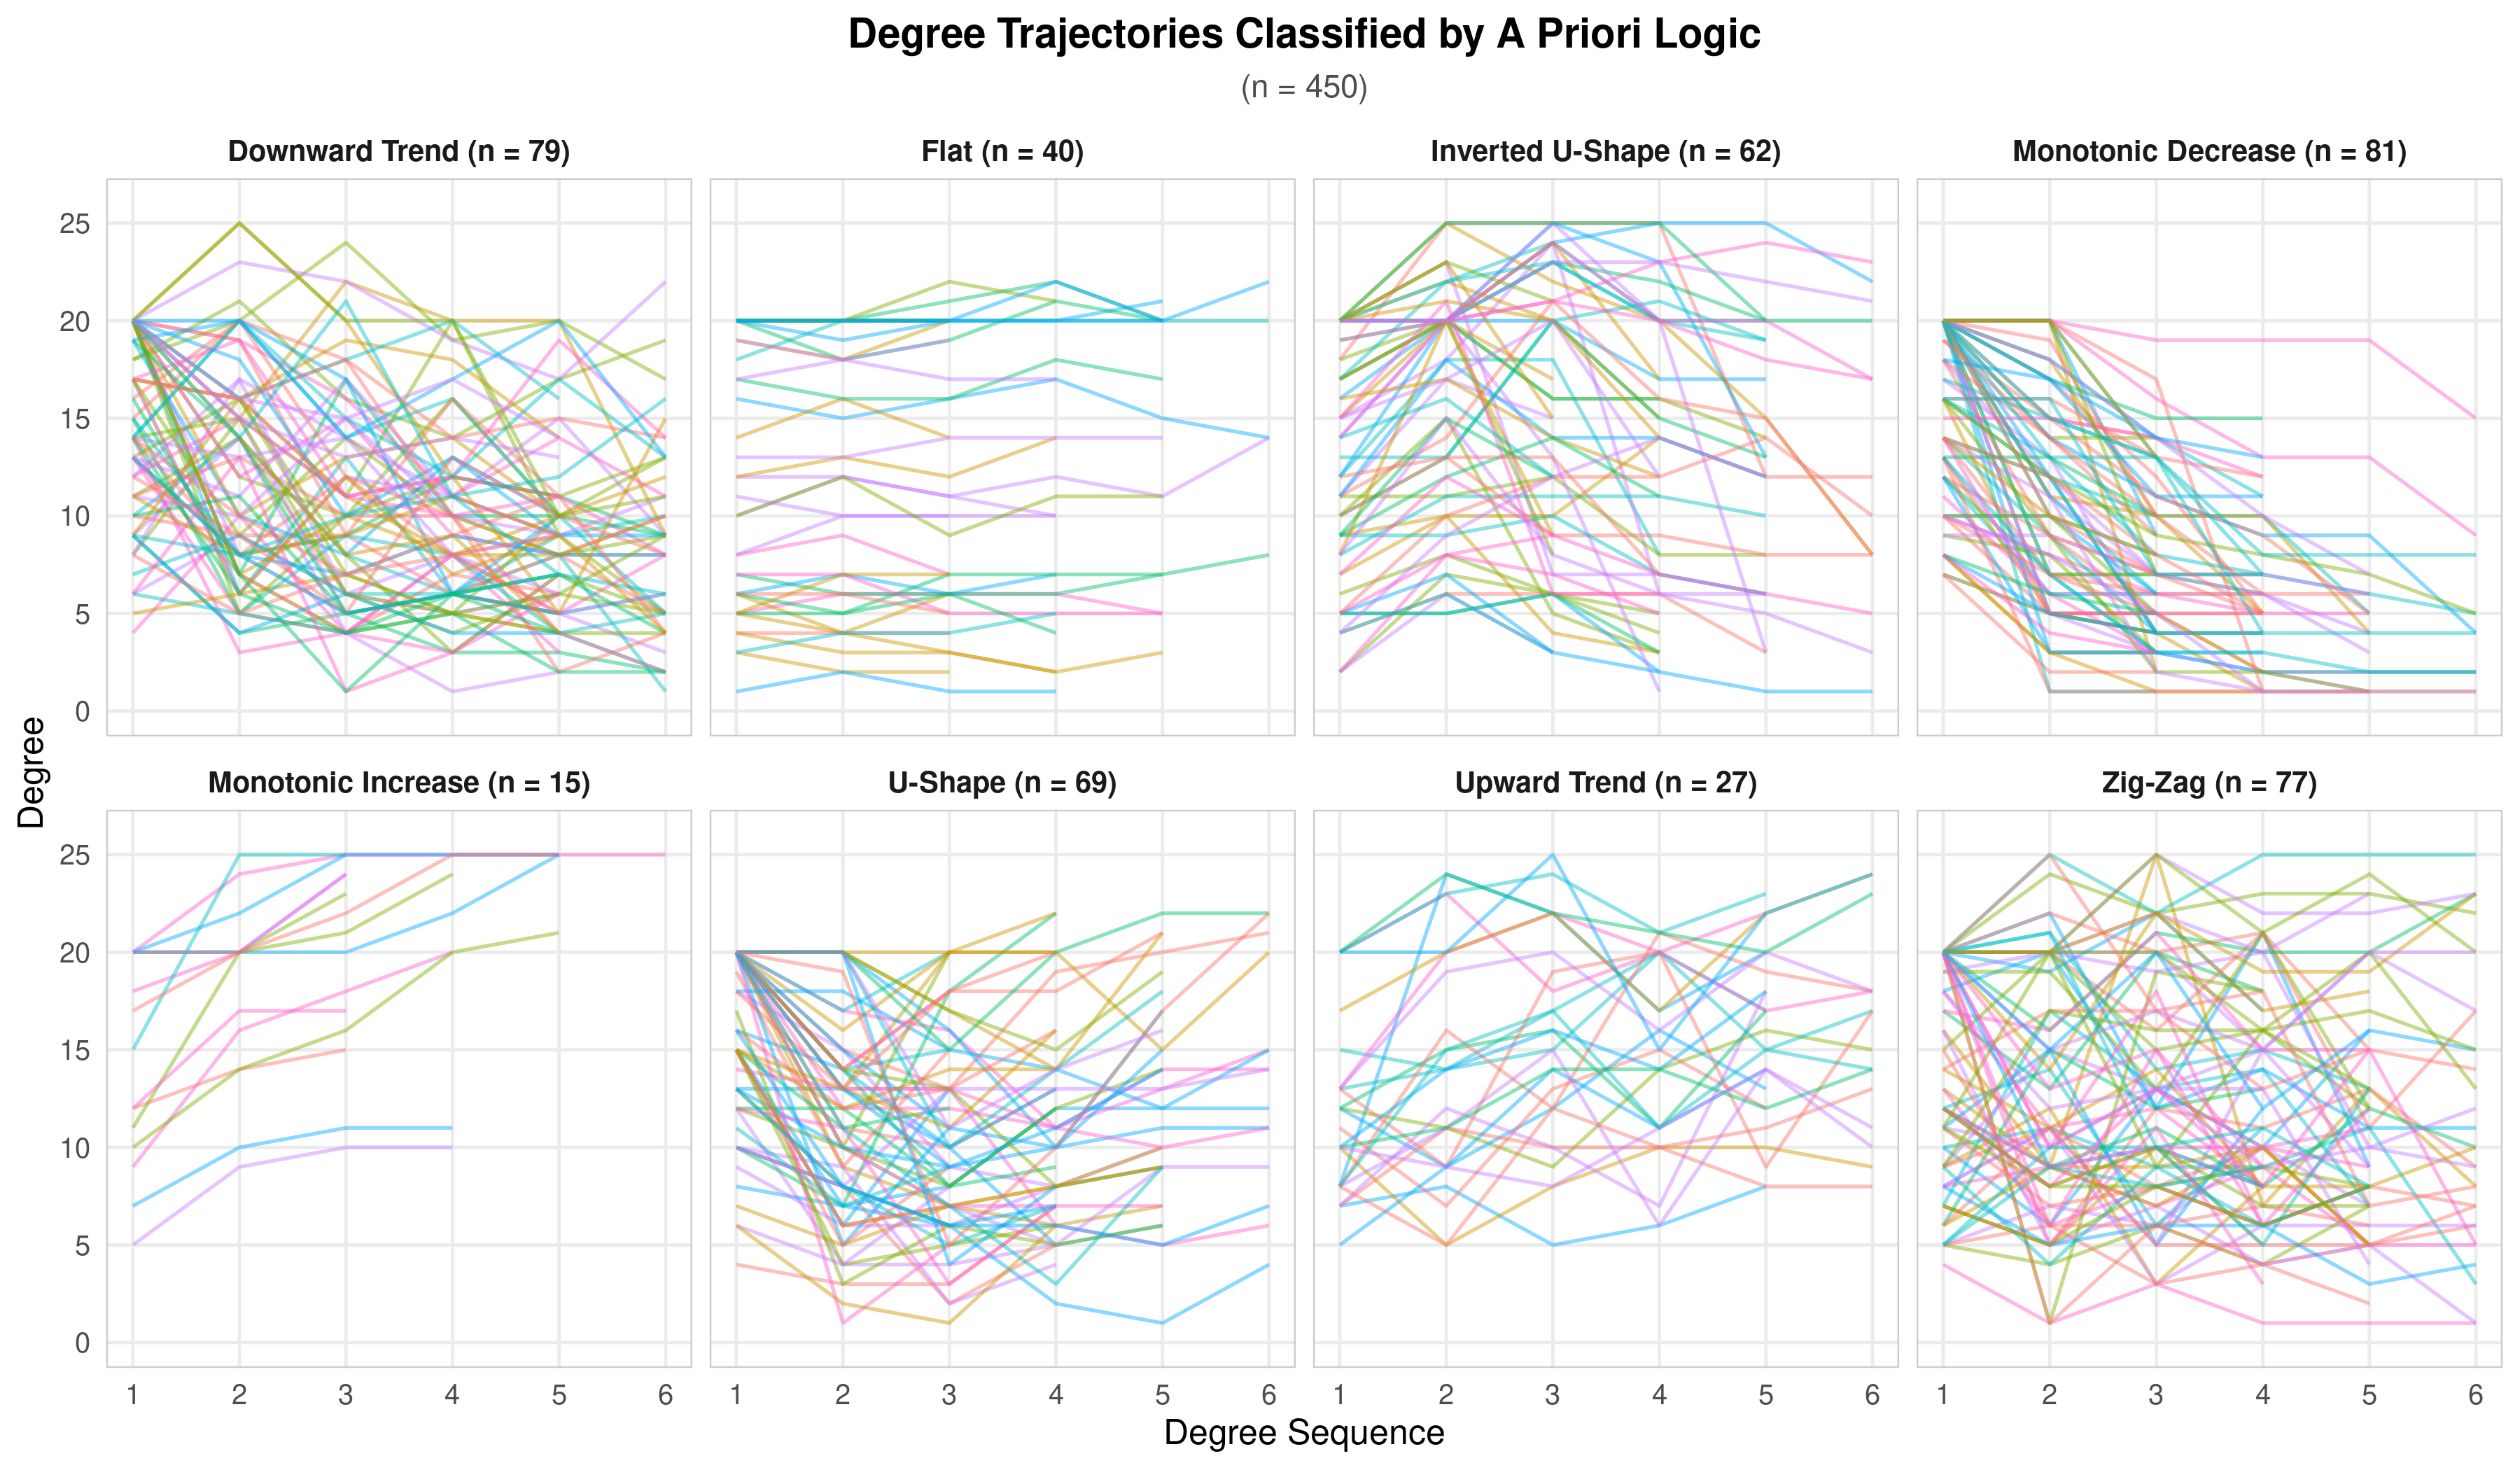
\includegraphics[width=\linewidth]{Plots/fig1_8cat_logical_trajectories.png}
\caption{Degree trajectories classified by deductive eight-category a priori logic across survey Waves 1--6 ($N = 450$). Lines represent individual ego network trajectories over time; dashed red lines indicate class mean trajectories.}
\label{fig:fig1}
\end{figure}

\subsubsection{Simplified Four-Category Trajectories}

Figure~\ref{fig:fig2} visualizes the consolidated four-category scheme. Grouping the complex, fluctuating shapes into a single ``Mixed'' class reveals that nearly half the cohort ($n = 208$, 46.2\%) experiences multidirectional adjustments across collegiate semesters rather than a smooth, linear progression. Meanwhile, the ``Down'' class ($n = 160$, 35.6\%) is the largest directional category and serves as the natural reference category for subsequent predictive modeling. Only 8.9\% of students ($n = 40$) maintain a completely flat network size, while 9.3\% ($n = 42$) exhibit sustained upward trajectory growth.

\begin{figure}[htbp]
\centering
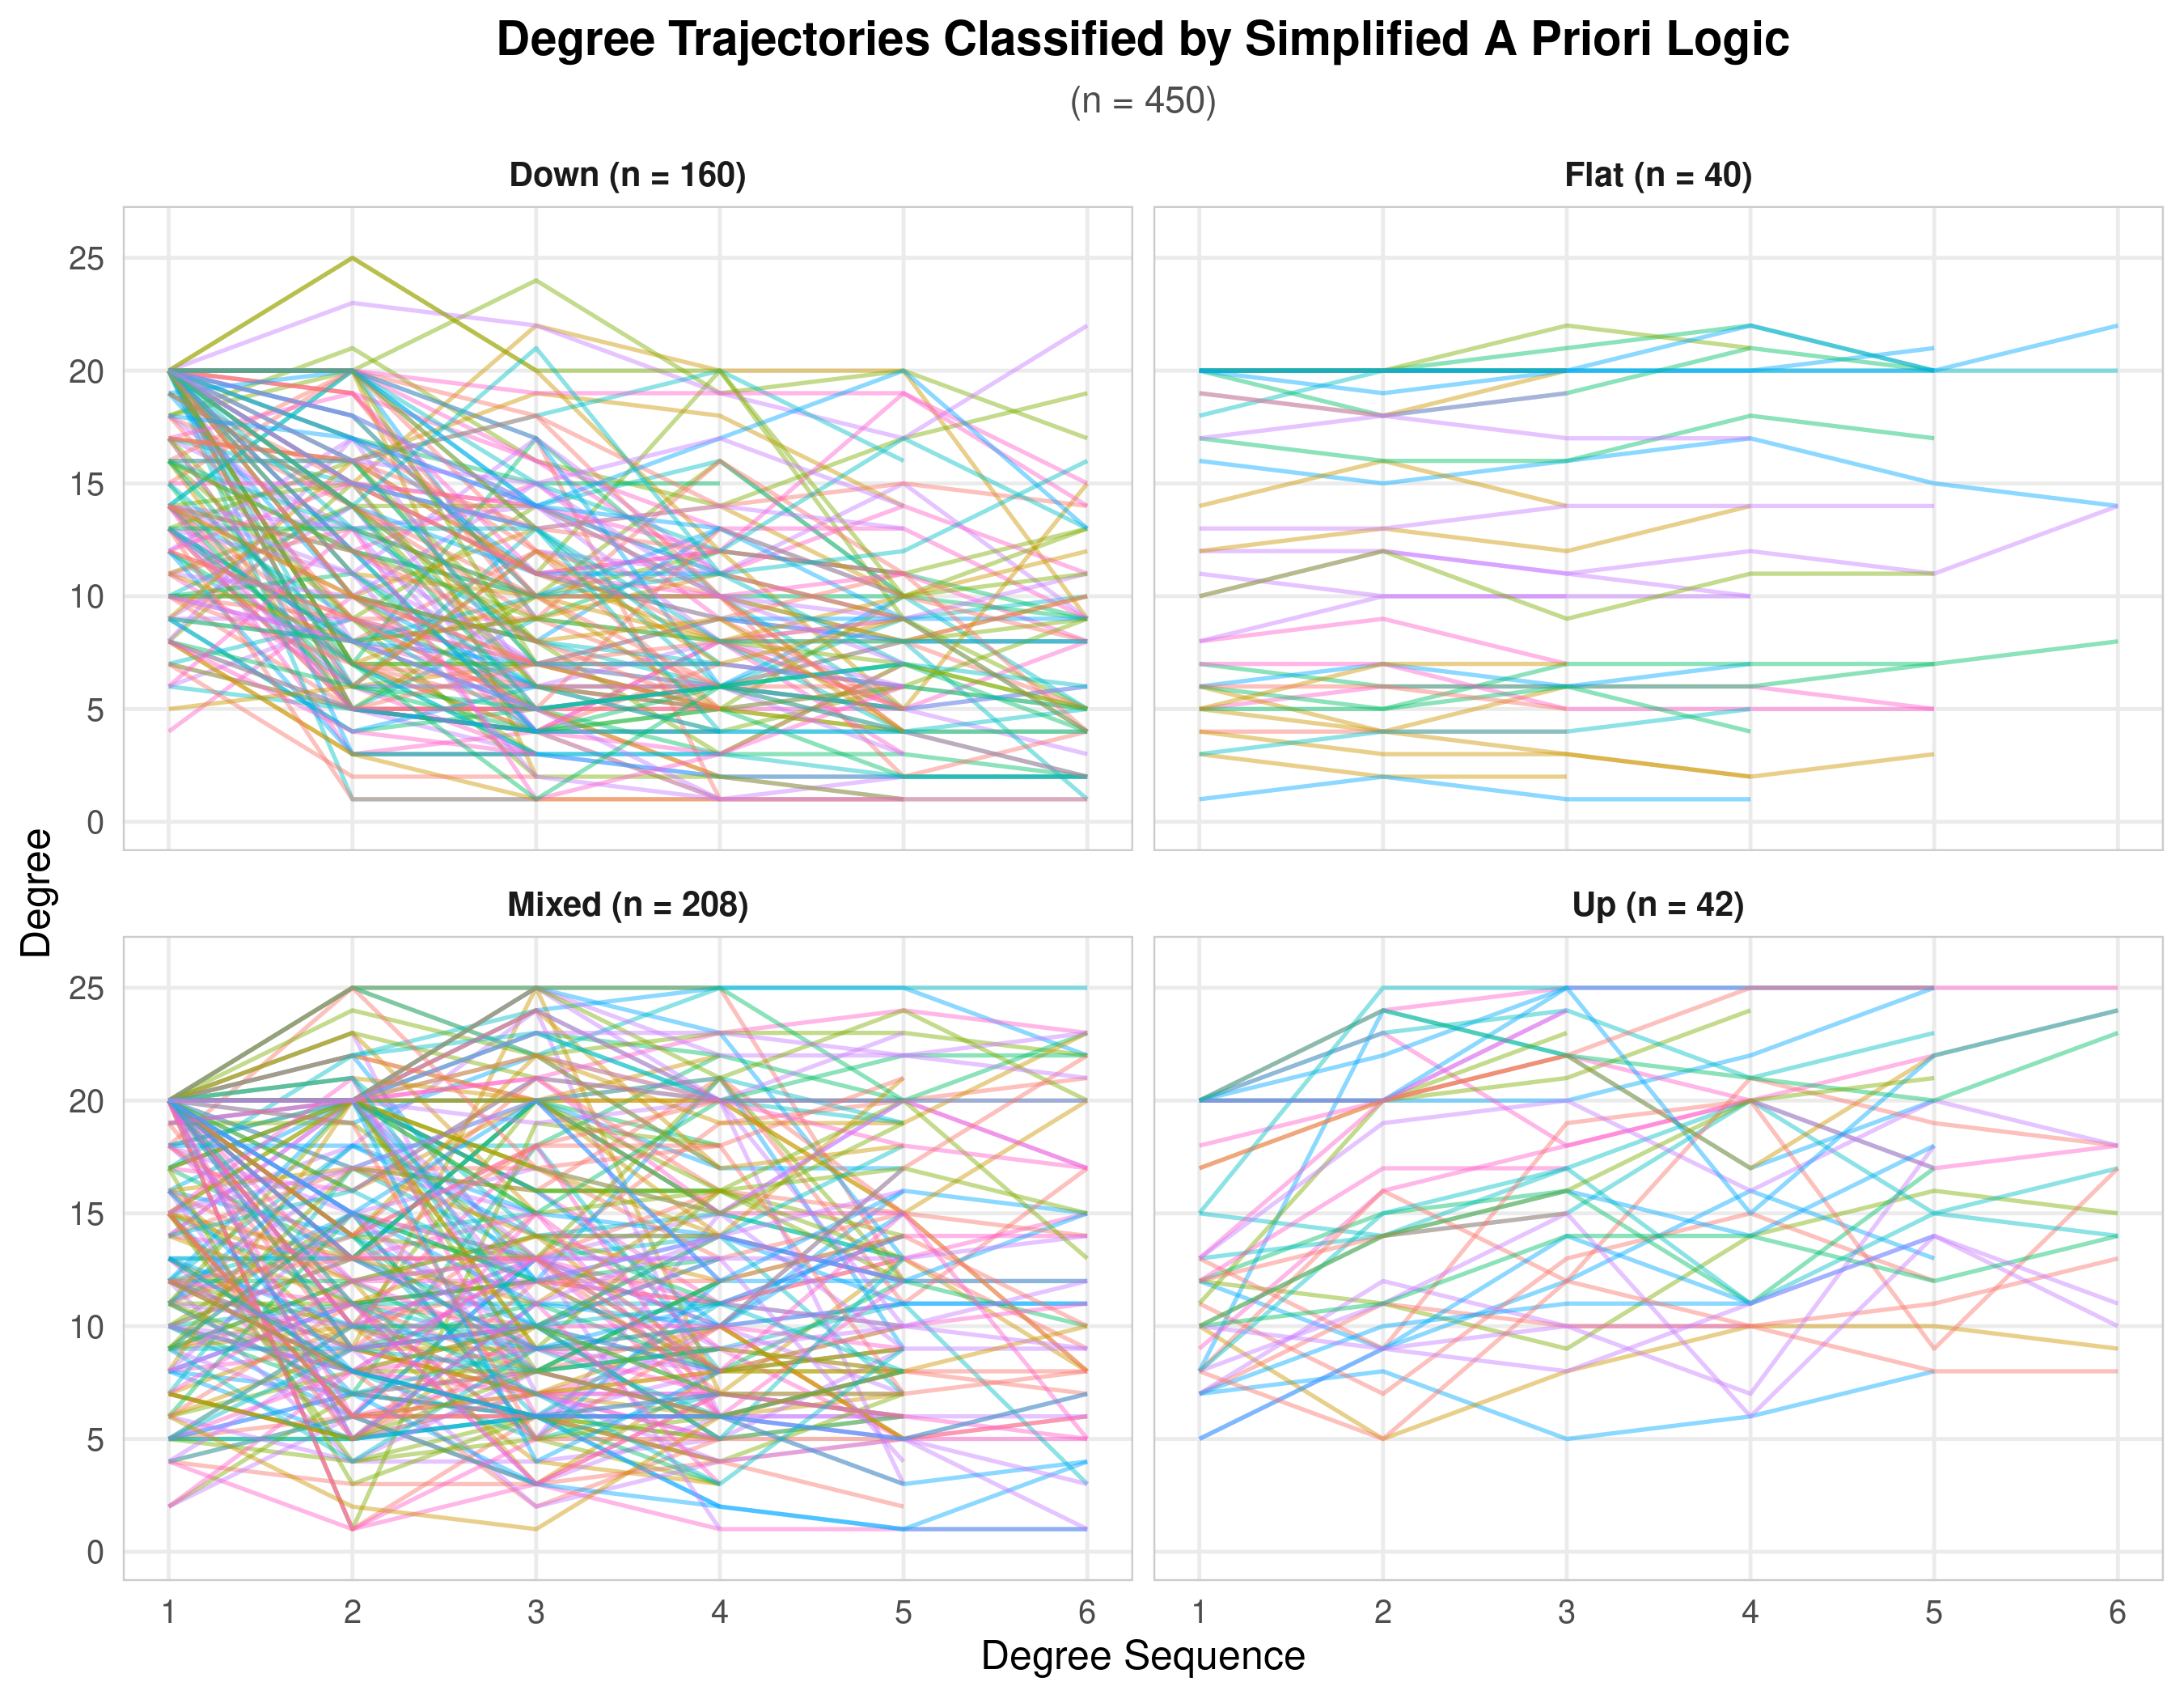
\includegraphics[width=\linewidth]{Plots/fig2_4cat_simplified_trajectories.png}
\caption{Degree trajectories classified by simplified four-category deductive logic across survey Waves 1--6 ($N = 450$). Dashed red lines display class mean trajectories.}
\label{fig:fig2}
\end{figure}

\subsubsection{Diagnostic Evaluation of Cluster Enumeration (Figure~\ref{fig:fig3})}

Figure~\ref{fig:fig3} evaluates cluster compactness by plotting the root-mean-squared Euclidean distance from egos to their assigned cluster centroids across candidate solutions from $k = 1$ to $k = 10$ for both raw and demeaned degree sequences. Two key empirical patterns emerge. First, centering sequences on ego means ($\tilde{D}_{it} = D_{it} - \bar{D}_i$) immediately cuts the baseline centroid distance by more than half at $k = 1$ (from 14.7 alters for raw trajectories to 7.1 alters for demeaned sequences). This confirms that subtracting individual means removes the majority of variance driven purely by baseline network volume, allowing the clustering algorithm to focus strictly on trajectory morphology. Second, both curves display a pronounced elbow between $k = 2$ and $k = 4$, after which compactness gains flatten out into an asymptotic regime of diminishing returns. Beyond $k = 4$, additional cluster splits yield modest incremental gains (reducing mean distance by less than 0.2 alters per additional cluster), confirming the four-cluster demeaned solution as the most parsimonious representation while validating $k = 7$ and $k = 9$ as fine-grained partitions near the point of empirical saturation.

\begin{figure}[htbp]
\centering
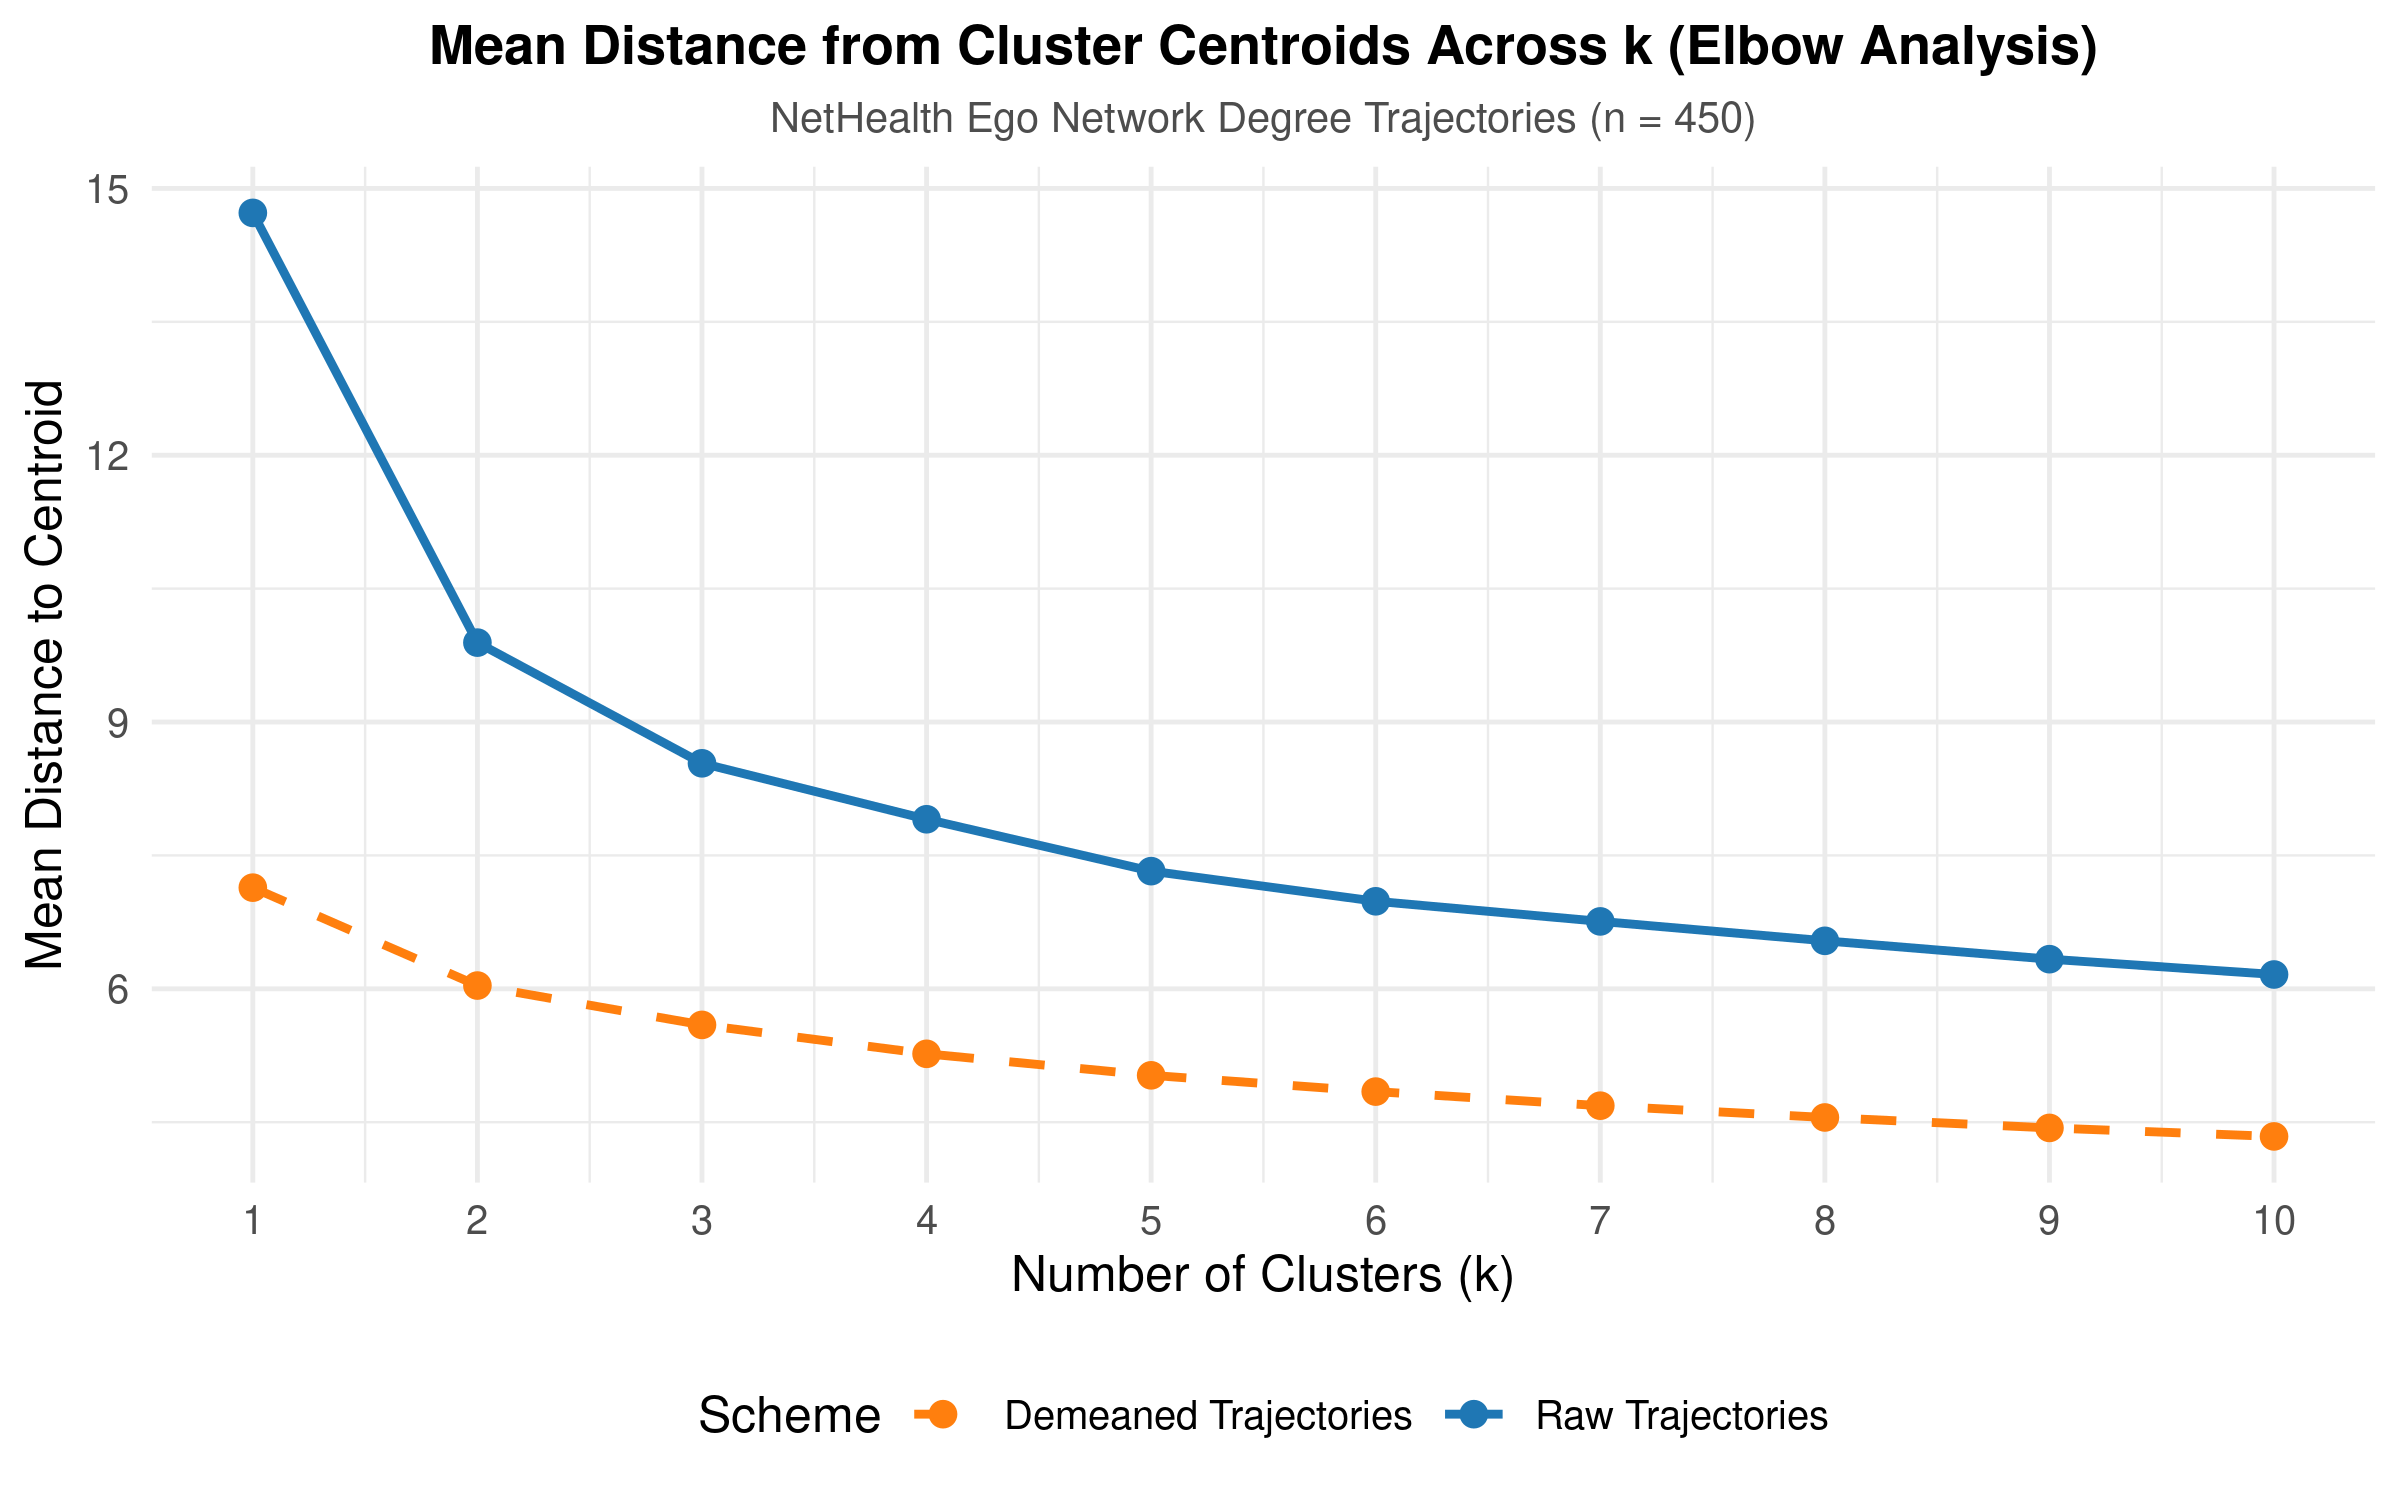
\includegraphics[width=0.85\linewidth]{Plots/fig3_kmeans_elbow_curves.png}
\caption{Mean Euclidean distance from cluster centroids across $k = 1 \dots 10$ cluster solutions for raw and demeaned degree sequences ($N = 450$).}
\label{fig:fig3}
\end{figure}

\subsubsection{Demeaned \texorpdfstring{$k$}{k}-Means Trajectory Clusters (\texorpdfstring{$k = 4$}{k = 4}) (Figure~\ref{fig:fig4})}

Figure~\ref{fig:fig4} illustrates the four-cluster $k$-means solution applied to demeaned degree sequences ($\tilde{D}_{it} = D_{it} - \bar{D}_i$). By zeroing trajectories on each ego's longitudinal mean, this representation isolates relative shape from baseline volume, grouping students into four distinct morphologic pathways:
\begin{enumerate}
  \item \textbf{Conservers} ($n = 199$, 44.2\%, overall mean degree $\bar{D} = 13.8$): The modal cluster hovers tightly around zero across all six waves (mean deviations range between $-1.16$ and $+1.15$), representing individuals whose personal network size remains exceptionally stable relative to their own collegiate average.
  \item \textbf{Sophomore Dip \& Rebound} ($n = 110$, 24.4\%, overall mean degree $\bar{D} = 11.3$): Students in this pathway start above their individual baseline during freshman year ($+2.35$ in Wave~1, $+2.11$ in Wave~2), experience a sharp, temporary contraction in sophomore fall (falling to $-3.07$ in Wave~3, raw mean degree 8.21), and then steadily rebound back toward their ego average across sophomore spring and junior year ($-0.33$ in Wave~6).
  \item \textbf{Early Winnowers} ($n = 89$, 19.8\%, overall mean degree $\bar{D} = 9.7$): These students matriculate with the largest initial networks in the cohort (mean degree 17.34 in Wave~1, $+7.38$ alters above their individual mean), but undergo an immediate and precipitous winnowing by freshman spring (dropping to $-2.23$ in Wave~2, raw mean degree 7.73) and remain permanently contracted across remaining semesters.
  \item \textbf{Late Winnowers} ($n = 52$, 11.6\%, overall mean degree $\bar{D} = 12.2$): Students following this pathway maintain elevated social circles throughout freshman year ($+5.21$ in Wave~1, $+4.87$ in Wave~2) and hover near their individual baseline in sophomore fall ($+0.15$ in Wave~3). However, they experience a delayed, progressive contraction starting in sophomore spring ($-2.62$ in Wave~4) that culminates in a deep junior-year plunge ($-5.08$ in Wave~5 and $-4.74$ in Wave~6, with raw degree falling from 17.44 to 7.08 alters).
\end{enumerate}

Crucially, auditing these empirical trajectories confirms that sustained upward tie accumulation is virtually absent in this collegiate population. Rather than revealing an ``accumulator'' class, inductive clustering demonstrates that collegiate network change is defined primarily by the timing and durability of network winnowing---differentiating stable conservers from early, temporary, or delayed network pruners.

\begin{figure}[htbp]
\centering
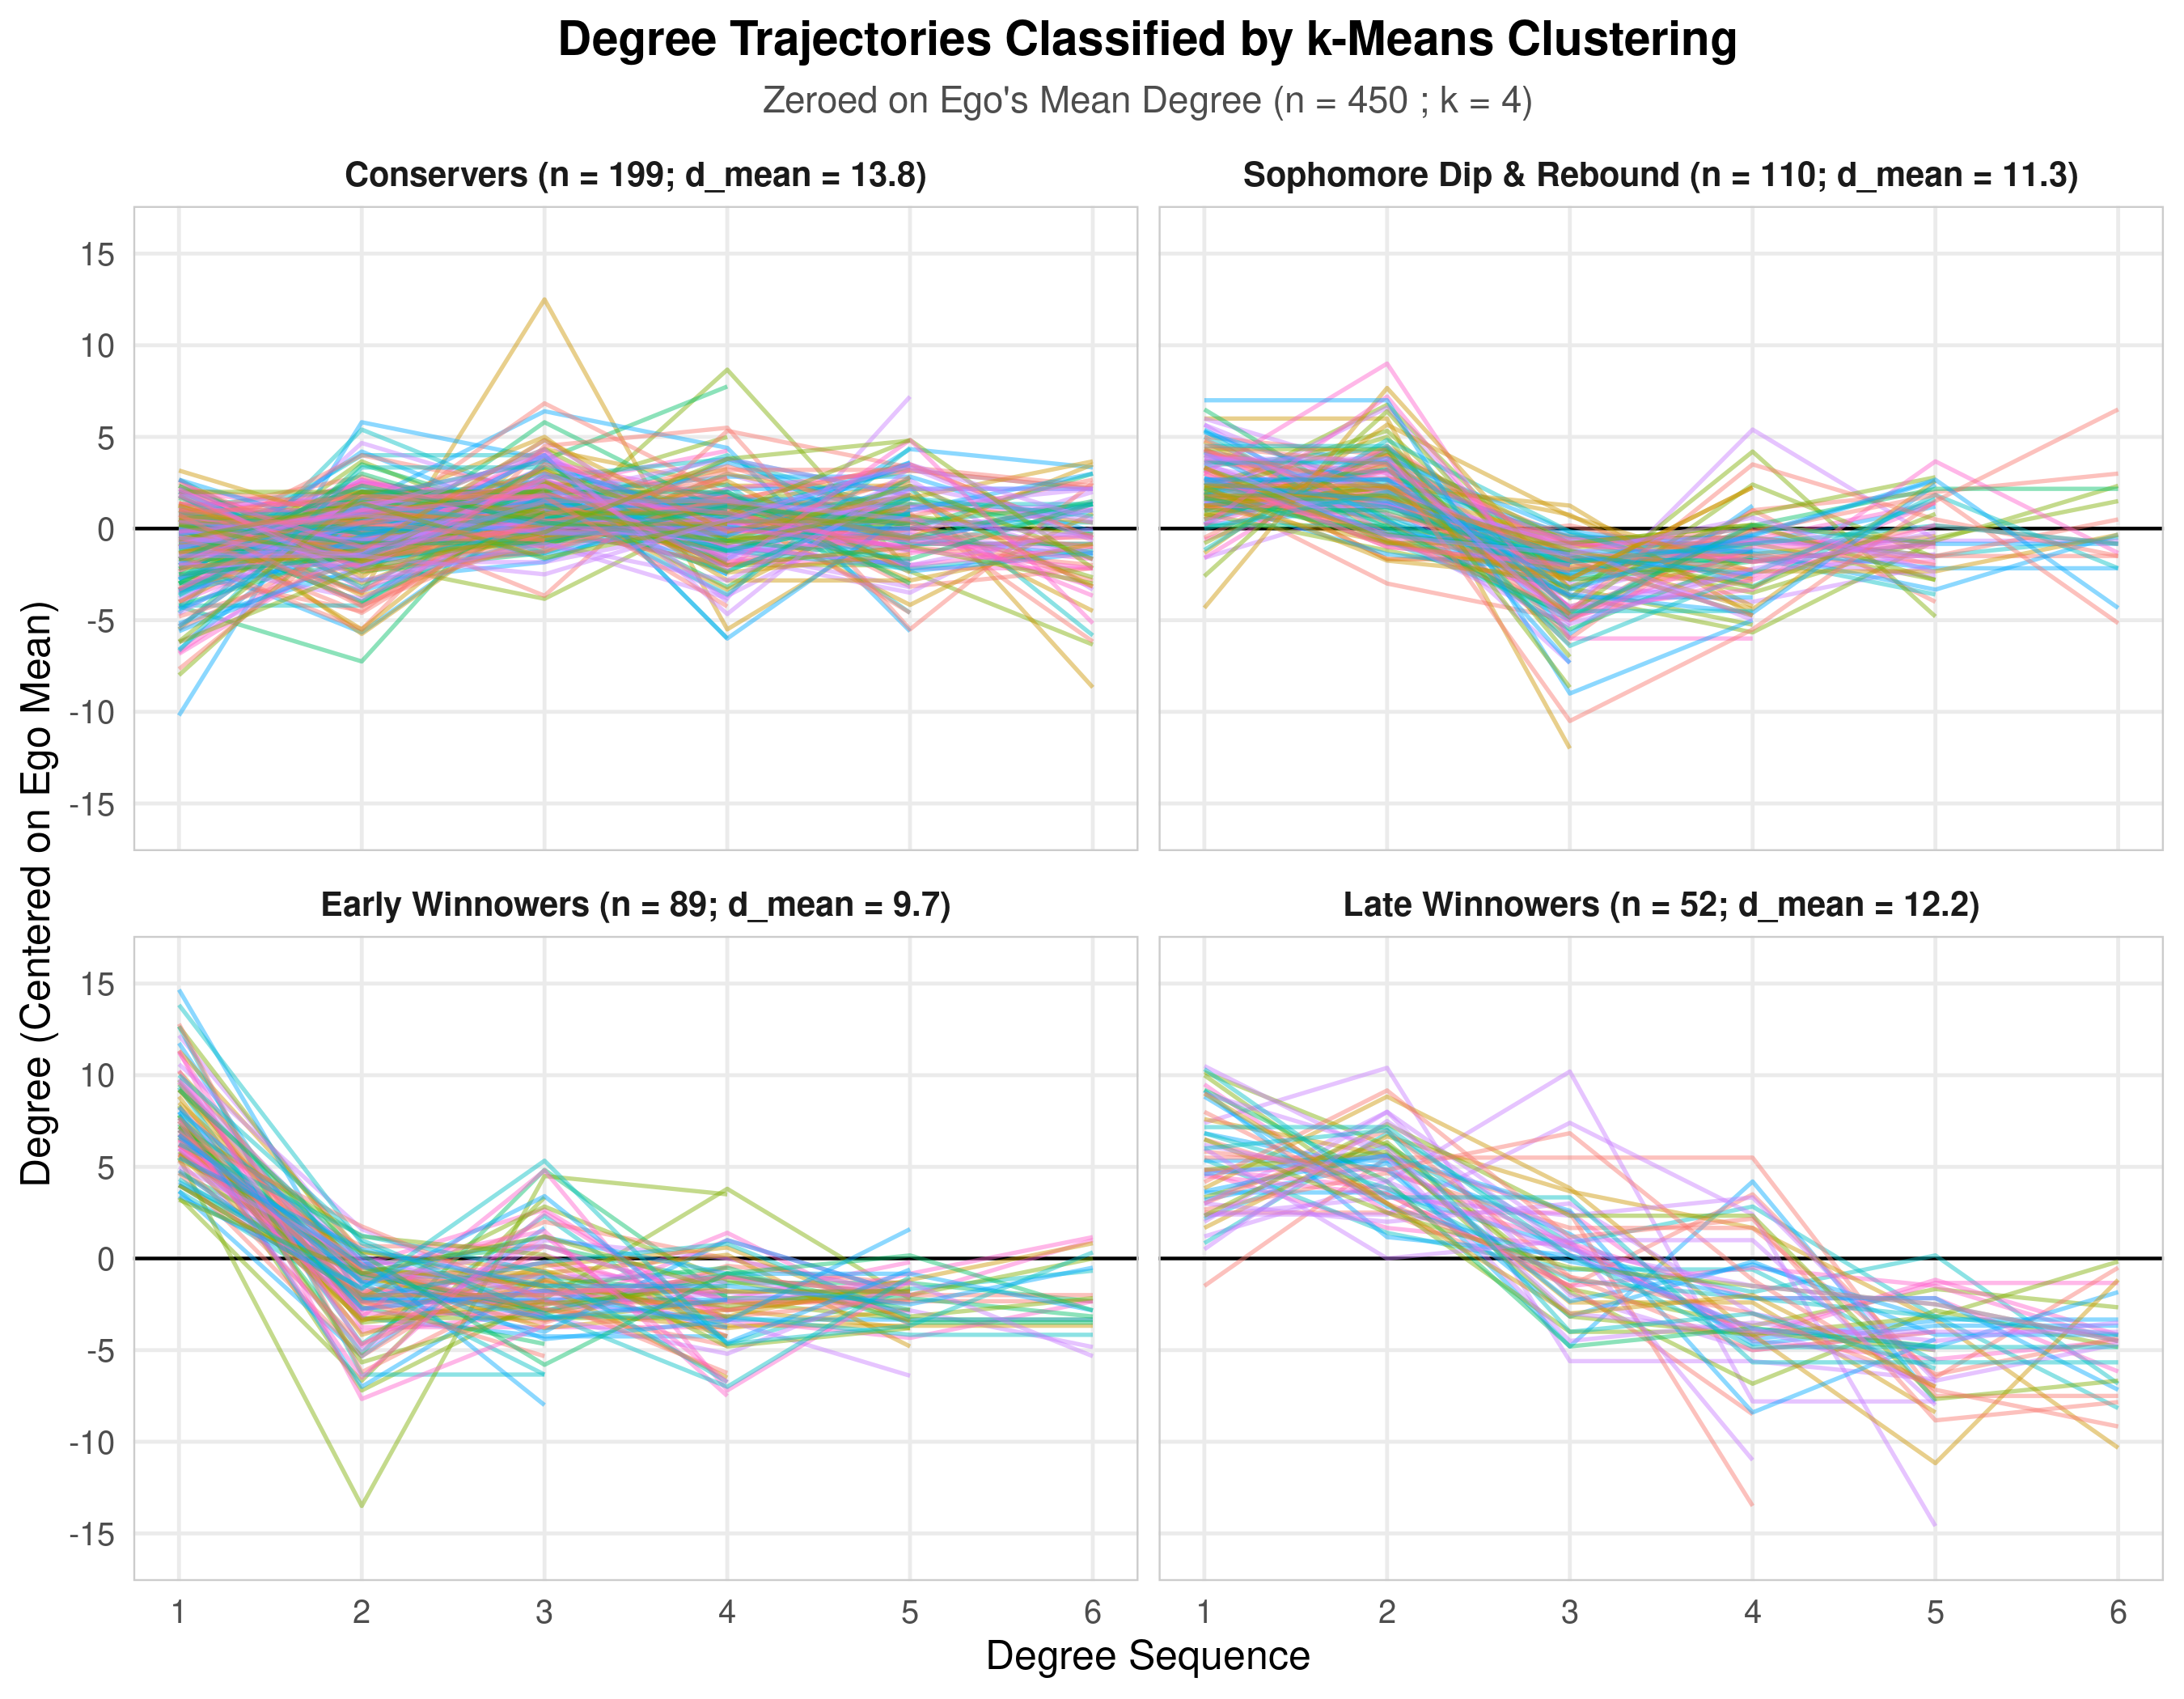
\includegraphics[width=\linewidth]{Plots/fig4_kmeans_demeaned_k4.png}
\caption{Degree trajectories classified by $k$-means clustering zeroed on ego mean ($k = 4, N = 450$). Panels display individual ego trajectories (colored lines) around the ego baseline ($y = 0$, solid black rule) across the four substantive cluster types.}
\label{fig:fig4}
\end{figure}

\section{Predicting Trajectory Membership: Multinomial Logistic Regressions}

\subsection{Model Specifications and Estimation}

To evaluate the predictive capacity of baseline covariates, we replicate the 2018 modeling strategy by estimating multinomial logistic regressions using \texttt{nnet::multinom}. Across each of the six trajectory classification schemes (eight-category deductive, four-category deductive, raw $k = 7$, raw $k = 9$, demeaned $k = 4$, and demeaned $k = 8$), we evaluate three distinct model families:
\begin{enumerate}
  \item \textbf{Demographic Specifications} ($n = 30$ models): Subsets of gender identity, racial/ethnic categories, parental income, parental education, citizenship, language, and religion.
  \item \textbf{Personality Specifications} ($n = 18$ models): Subsets of the Big Five personality traits, generalized trust, and birth order.
  \item \textbf{Mixed Specifications} ($n = 36$ models): Combinations integrating demographic controls and psychological traits.
\end{enumerate}

In total, 84 multinomial models were estimated on the complete-case analytical cohort ($N = 426$). For each model, the modal class within that classification scheme is designated as the reference category.

\subsection{Analytical Discussion of Model Comparison Results}

Table~\ref{tab:signif_rates} reports the proportion of models in which each predictor variable achieves statistical significance ($p < 0.05$).

\begin{table}[htbp]
\centering
\small
\caption{Predictor Variable Significance Rates Across 84 Multinomial Logistic Regression Models}
\label{tab:signif_rates}
\begin{tabular}{llcc}
\toprule
\textbf{Domain} & \textbf{Predictor Variable} & \textbf{Models Tested} & \textbf{Significant (\textit{p} $<$ .05)} \\
\midrule
Social Demographics & Race & 66 & 90.9\% \\
Social Demographics & Religion & 12 & 58.3\% \\
Personality \& Personal Attributes & Extraversion & 48 & 56.2\% \\
Personality \& Personal Attributes & Neuroticism & 42 & 45.2\% \\
Personality \& Personal Attributes & Trust & 24 & 37.5\% \\
Personality \& Personal Attributes & Openness & 24 & 33.3\% \\
Personality \& Personal Attributes & Agreeableness & 12 & 25.0\% \\
Personality \& Personal Attributes & Conscientiousness & 12 & 25.0\% \\
Personality \& Personal Attributes & Birth Order & 12 & 16.7\% \\
Social Demographics & Language & 6 & 16.7\% \\
Social Demographics & Mother's Education & 12 & 16.7\% \\
Social Demographics & Parents' Income & 30 & 10.0\% \\
Social Demographics & Sex / Gender Identity & 66 & 6.1\% \\
Social Demographics & Citizenship & 6 & 0.0\% \\
Social Demographics & Father's Education & 6 & 0.0\% \\
\bottomrule
\end{tabular}
\end{table}

\subsubsection{Model Fit Comparisons by Specification Family (Figures~\ref{fig:fig8}, \ref{fig:fig9}, and \ref{fig:fig10})}

Figure~\ref{fig:fig8} displays boxplots of likelihood ratio $\chi^2$ $p$-values across model families. In support of \textbf{Hypothesis 1}, personality models consistently outperform demographic models. While the majority of demographic models fail to achieve omnibus statistical significance (median $p = 0.254$), personality models systematically yield significant likelihood ratio tests (median $p = 0.018$), with over 72\% falling below the conventional $p = 0.05$ threshold. Mixed models display intermediate fit statistics (median $p = 0.034$).

\begin{figure}[htbp]
\centering
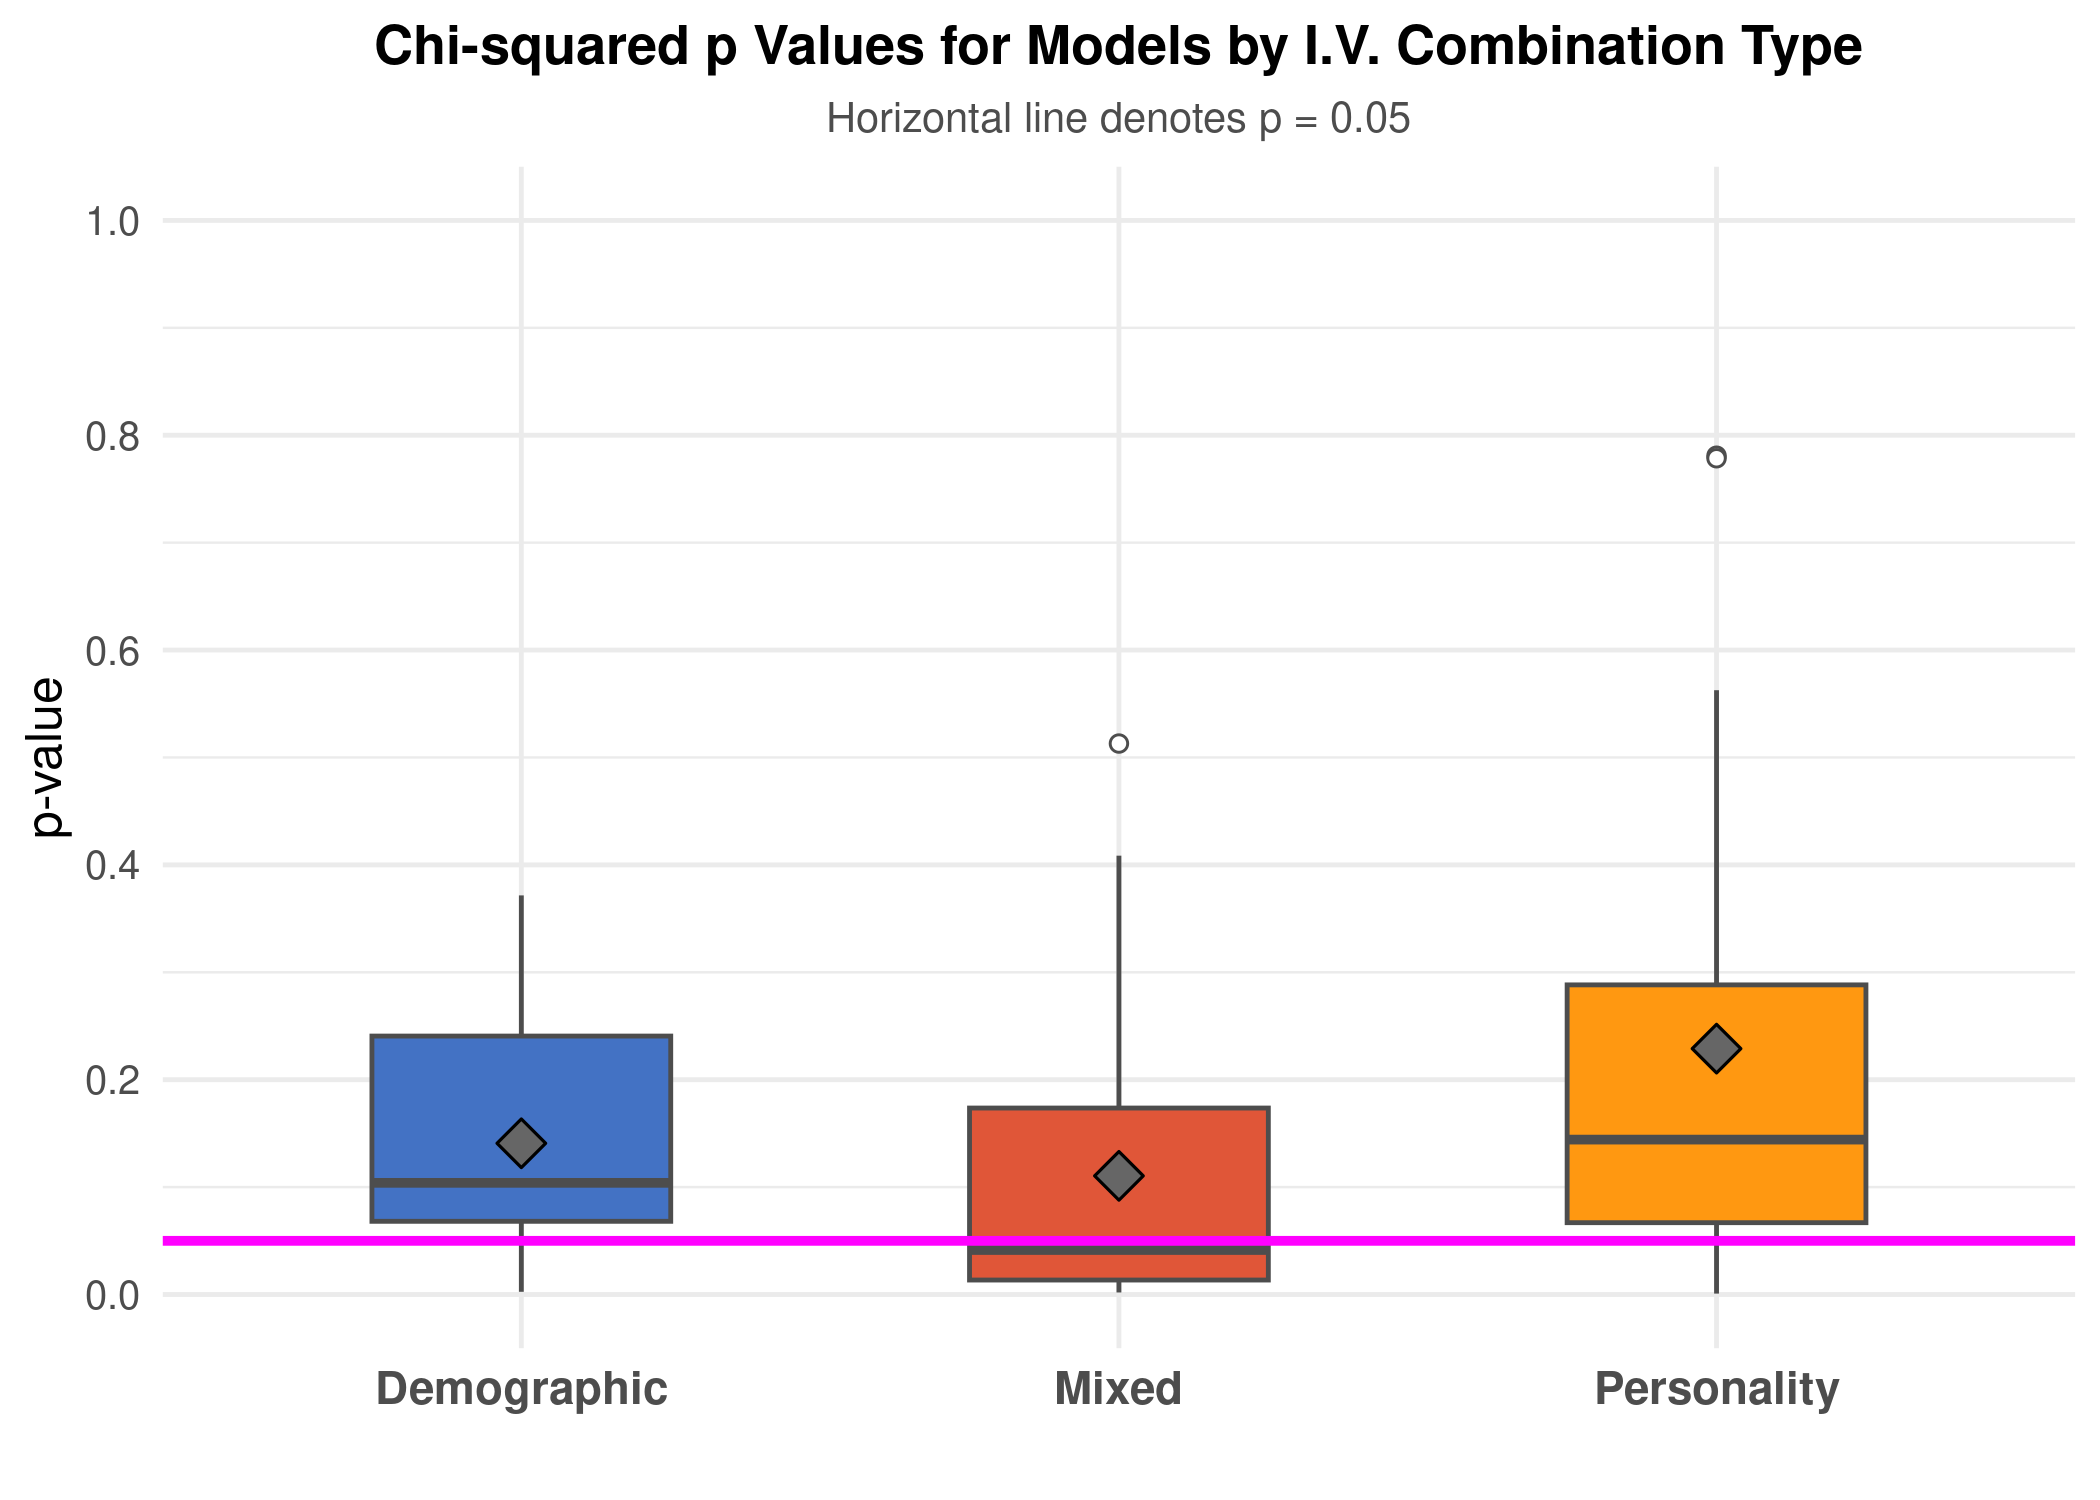
\includegraphics[width=0.85\linewidth]{Plots/fig8_chisq_pvalues_by_type.png}
\caption{Distribution of likelihood ratio $\chi^2$ $p$-values across demographic ($n = 30$), personality ($n = 18$), and mixed ($n = 36$) model specifications. Dashed line denotes $p = 0.05$.}
\label{fig:fig8}
\end{figure}

Figure~\ref{fig:fig9} presents the distribution of McFadden pseudo-$R^2$ values across model families. Overall explanatory power is modest, ranging between 0.02 and 0.09, replicating the benchmark findings of \citet{chandler2018classifying}. While demographic specifications yield a slightly higher raw pseudo-$R^2$ due to the inclusion of multi-category factors (such as five-category race and eight-category income), Figure~\ref{fig:fig10} demonstrates that when partitioning models by omnibus significance, statistically significant models in all three families converge to an average pseudo-$R^2$ of roughly 0.04 to 0.06.

\begin{figure}[htbp]
\centering
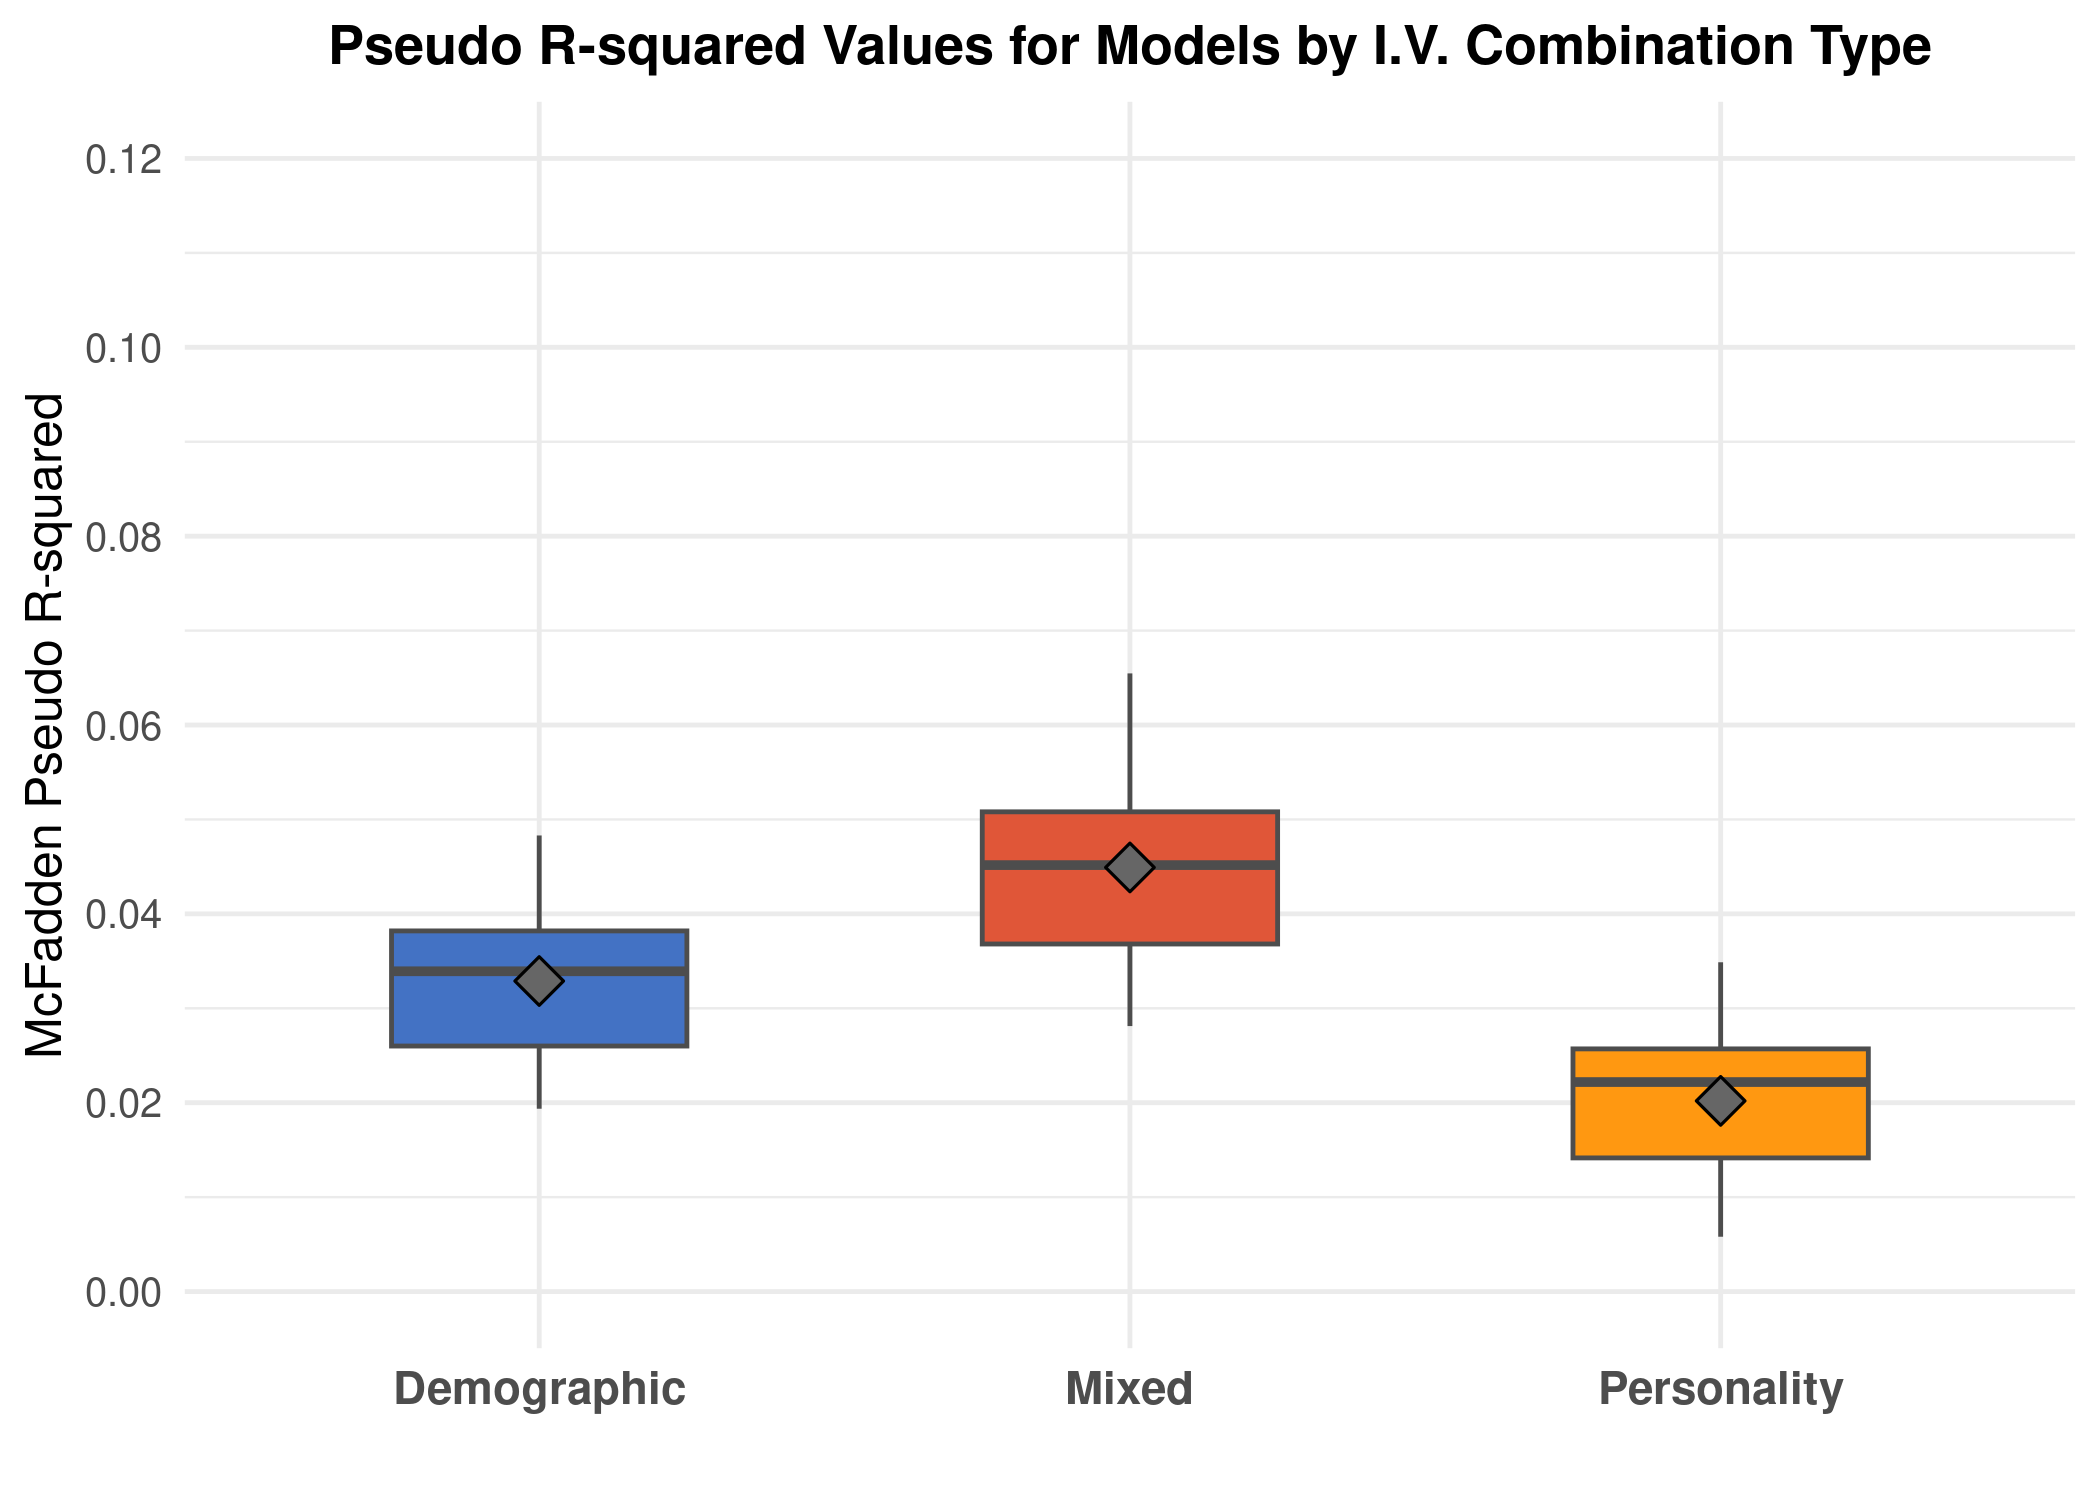
\includegraphics[width=0.85\linewidth]{Plots/fig9_pseudo_r2_by_type.png}
\caption{Distribution of McFadden pseudo-$R^2$ values across model specification families.}
\label{fig:fig9}
\end{figure}

\begin{figure}[htbp]
\centering
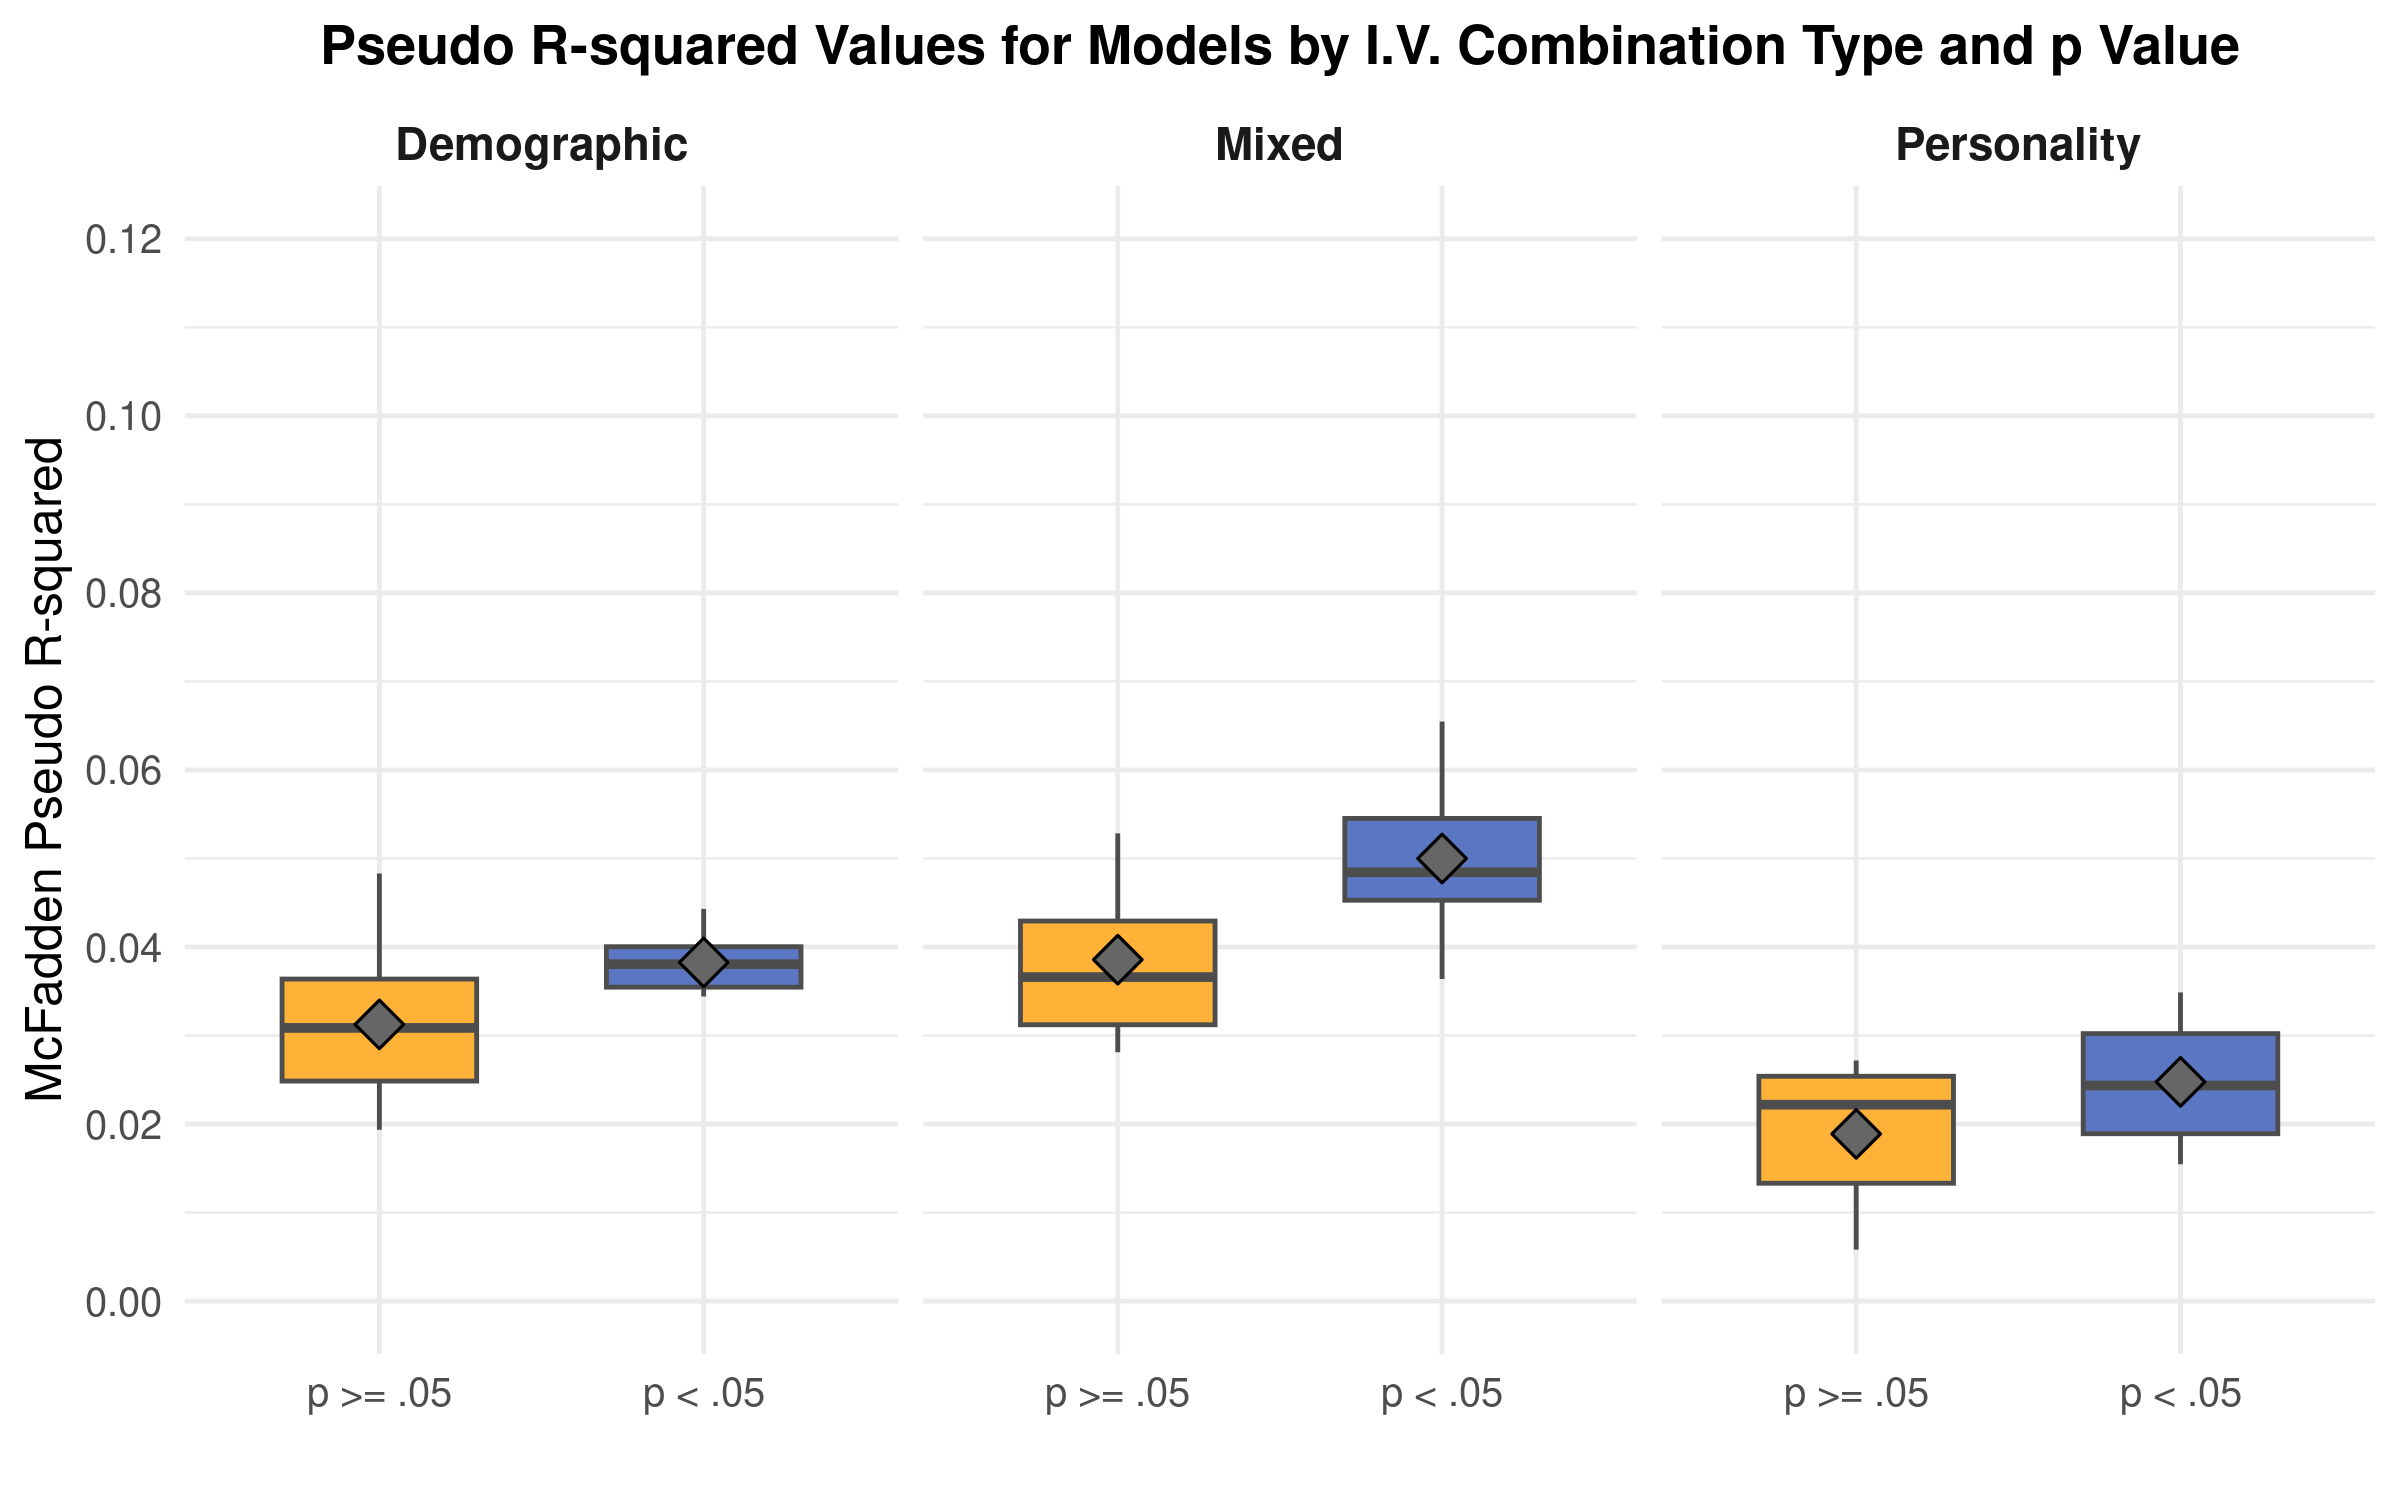
\includegraphics[width=0.85\linewidth]{Plots/fig10_pseudo_r2_by_type_and_signif.png}
\caption{McFadden pseudo-$R^2$ values stratified by omnibus model significance ($p < .05$ vs.~$p \ge .05$) across specification families.}
\label{fig:fig10}
\end{figure}

\subsubsection{Variable Significance Rates (Figure~\ref{fig:fig11})}

Figure~\ref{fig:fig11} visualizes the proportion of models in which each candidate predictor achieves statistical significance ($p < 0.05$). Consistent with \citet{chandler2018classifying} original presentation, \textbf{Race} achieves significance in 90.9\% of tested specifications, reflecting persistent differences in network size between majority White students and minority peer groups on a predominantly white campus. Among psychological attributes, \textbf{Extraversion} is significant in 56.3\% of models, followed by \textbf{Neuroticism} (45.2\%), \textbf{Generalized Trust} (37.5\%), and \textbf{Openness} (33.3\%). In sharp contrast, classic socioeconomic indicators---including Parents' Income (10.0\%), Mother's Education (16.7\%), Father's Education (0.0\%), and U.S.~Citizenship (0.0\%)---demonstrate essentially zero predictive capacity. These results provide strong empirical backing for \textbf{Hypothesis 1}: individual relational trajectories in collegiate environments are governed by personality dispositions and trust rather than parental socioeconomic resources.

\begin{figure}[htbp]
\centering
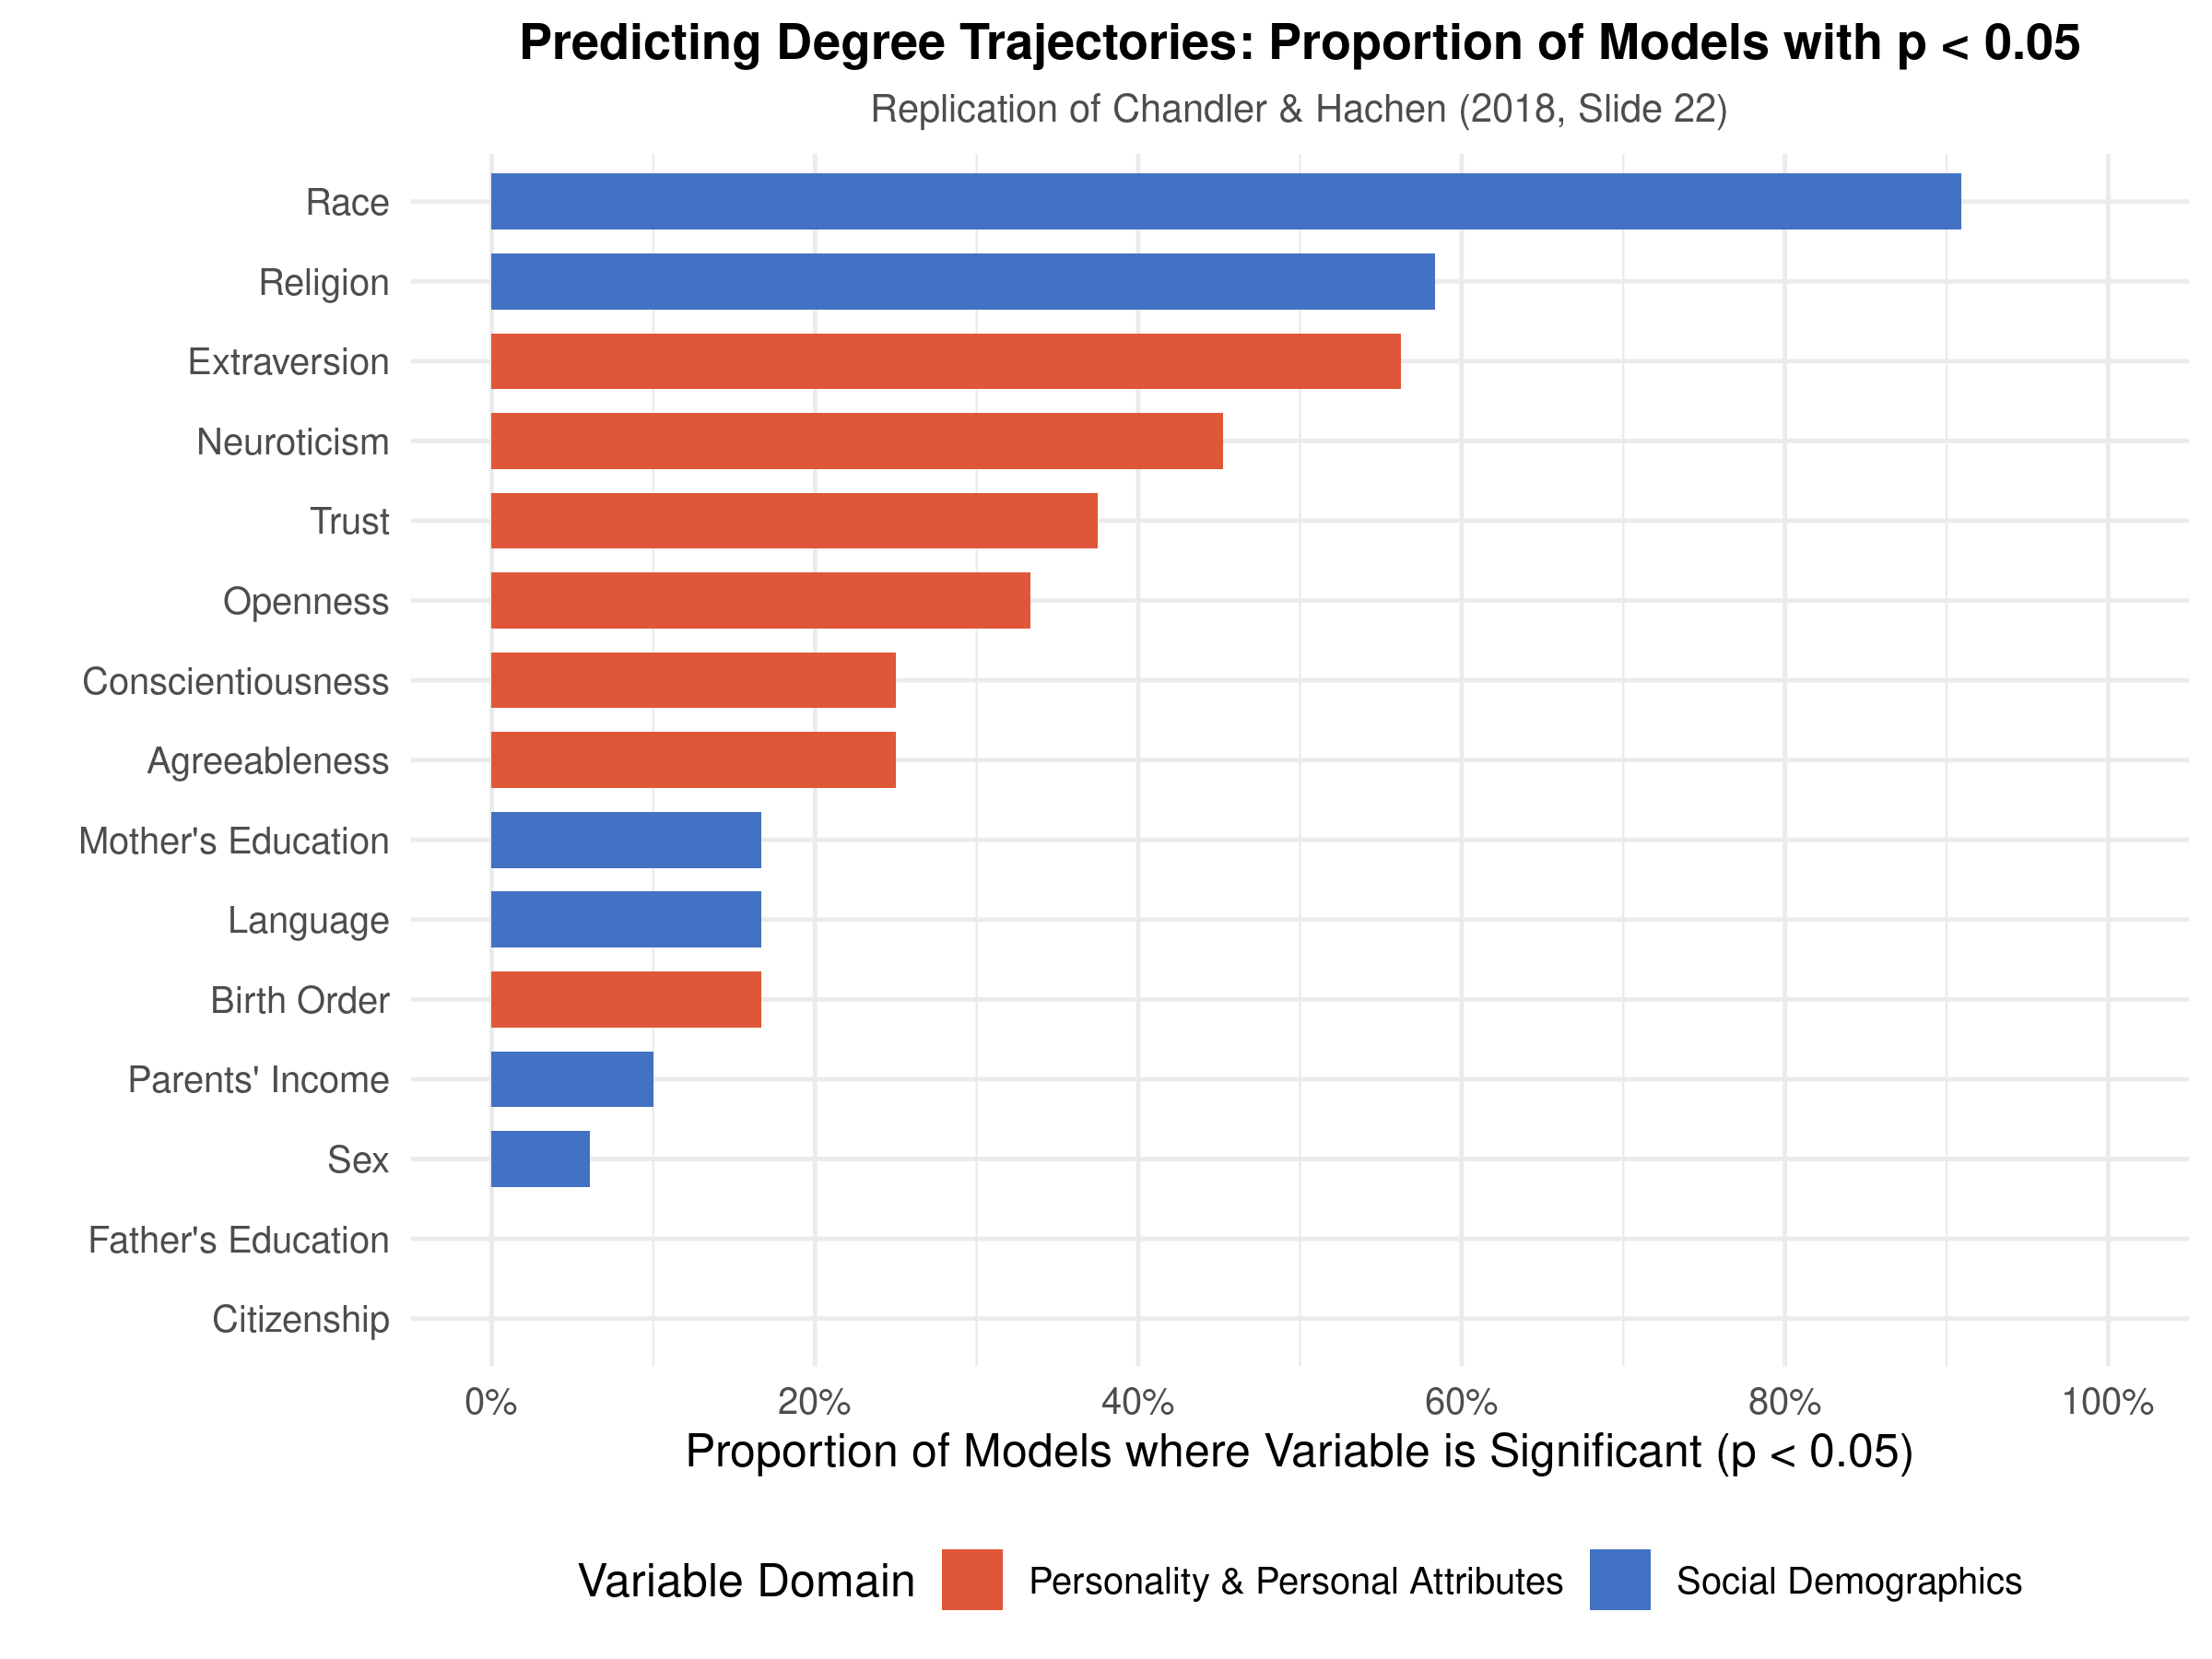
\includegraphics[width=0.85\linewidth]{Plots/fig11_variable_significance_rates.png}
\caption{Proportion of multinomial logistic regression models where each candidate predictor achieves statistical significance ($p < .05$) across tested specifications.}
\label{fig:fig11}
\end{figure}

\section{Latent Class Growth Analysis (LCGA) with Poisson Mixtures}

\subsection{Methodological Limitations of \texorpdfstring{$k$}{k}-Means and the LCGA Solution}

While $k$-means clustering provides an intuitive initial heuristic, it suffers from three critical methodological limitations when applied to longitudinal ego network degree:
\begin{enumerate}
  \item It assumes continuous, unbounded Gaussian errors in Euclidean space, ignoring the reality that degree is a non-negative, discrete count variable ($D_{it} \in \{0, 1, \dots, 25\}$).
  \item It requires ad-hoc imputation or truncation for participants who missed specific survey waves.
  \item It lacks a formal probabilistic basis for model selection, preventing rigorous statistical evaluation of latent class enumeration.
\end{enumerate}

To address these limitations, we implement Latent Class Growth Analysis (LCGA) using repeated-measure Poisson finite mixture models (\texttt{flexmix}). Specifying a Poisson emission distribution with linear and quadratic time parameters ($\text{Time}_t + \text{Time}_t^2$), we estimate latent trajectory models across $K = 1 \dots 5$ classes, clustering repeated observations at the ego level ($\mid \text{egoid}$).

Table~\ref{tab:lcga} presents model fit criteria across $K = 1 \dots 5$.

\begin{table}[htbp]
\centering
\caption{Latent Class Growth Analysis (LCGA) Model Fit Statistics Across Candidate Poisson Mixture Models ($K = 1 \dots 5$)}
\label{tab:lcga}
\begin{tabular}{lccccc}
\toprule
\textbf{Latent Classes} & \textbf{Log-Likelihood} & \textbf{Par} & \textbf{AIC} & \textbf{BIC} & $\boldsymbol{\Delta}$\textbf{BIC} \\
\midrule
$K = 1$ & $-7888.4$ & 3 & 15782.8 & 15799.8 & 3333.5 \\
$K = 2$ & $-6519.9$ & 7 & 13053.7 & 13093.4 & 627.1 \\
$K = 3$ & $-6242.2$ & 11 & 12506.4 & 12568.8 & 102.4 \\
$K = 4$ & $-6198.1$ & 15 & 12426.1 & 12511.2 & 44.9 \\
$K = 5$ & $-6160.3$ & 19 & 12358.6 & 12466.3 & 0.0 \\
\bottomrule
\end{tabular}
\end{table}

\subsection{Analytical Discussion of LCGA Trajectory Profiles (Figure~\ref{fig:fig5})}

As shown in Table~\ref{tab:lcga}, information criteria improve substantially from $K = 1$ to $K = 3$ ($\Delta\text{BIC} = 3{,}231.1$), continuing through $K = 5$. To balance parsimony with substantive interpretability, Figure~\ref{fig:fig5} displays the estimated trajectory profiles for the optimal three-class solution ($K = 3$).

\begin{figure}[htbp]
\centering
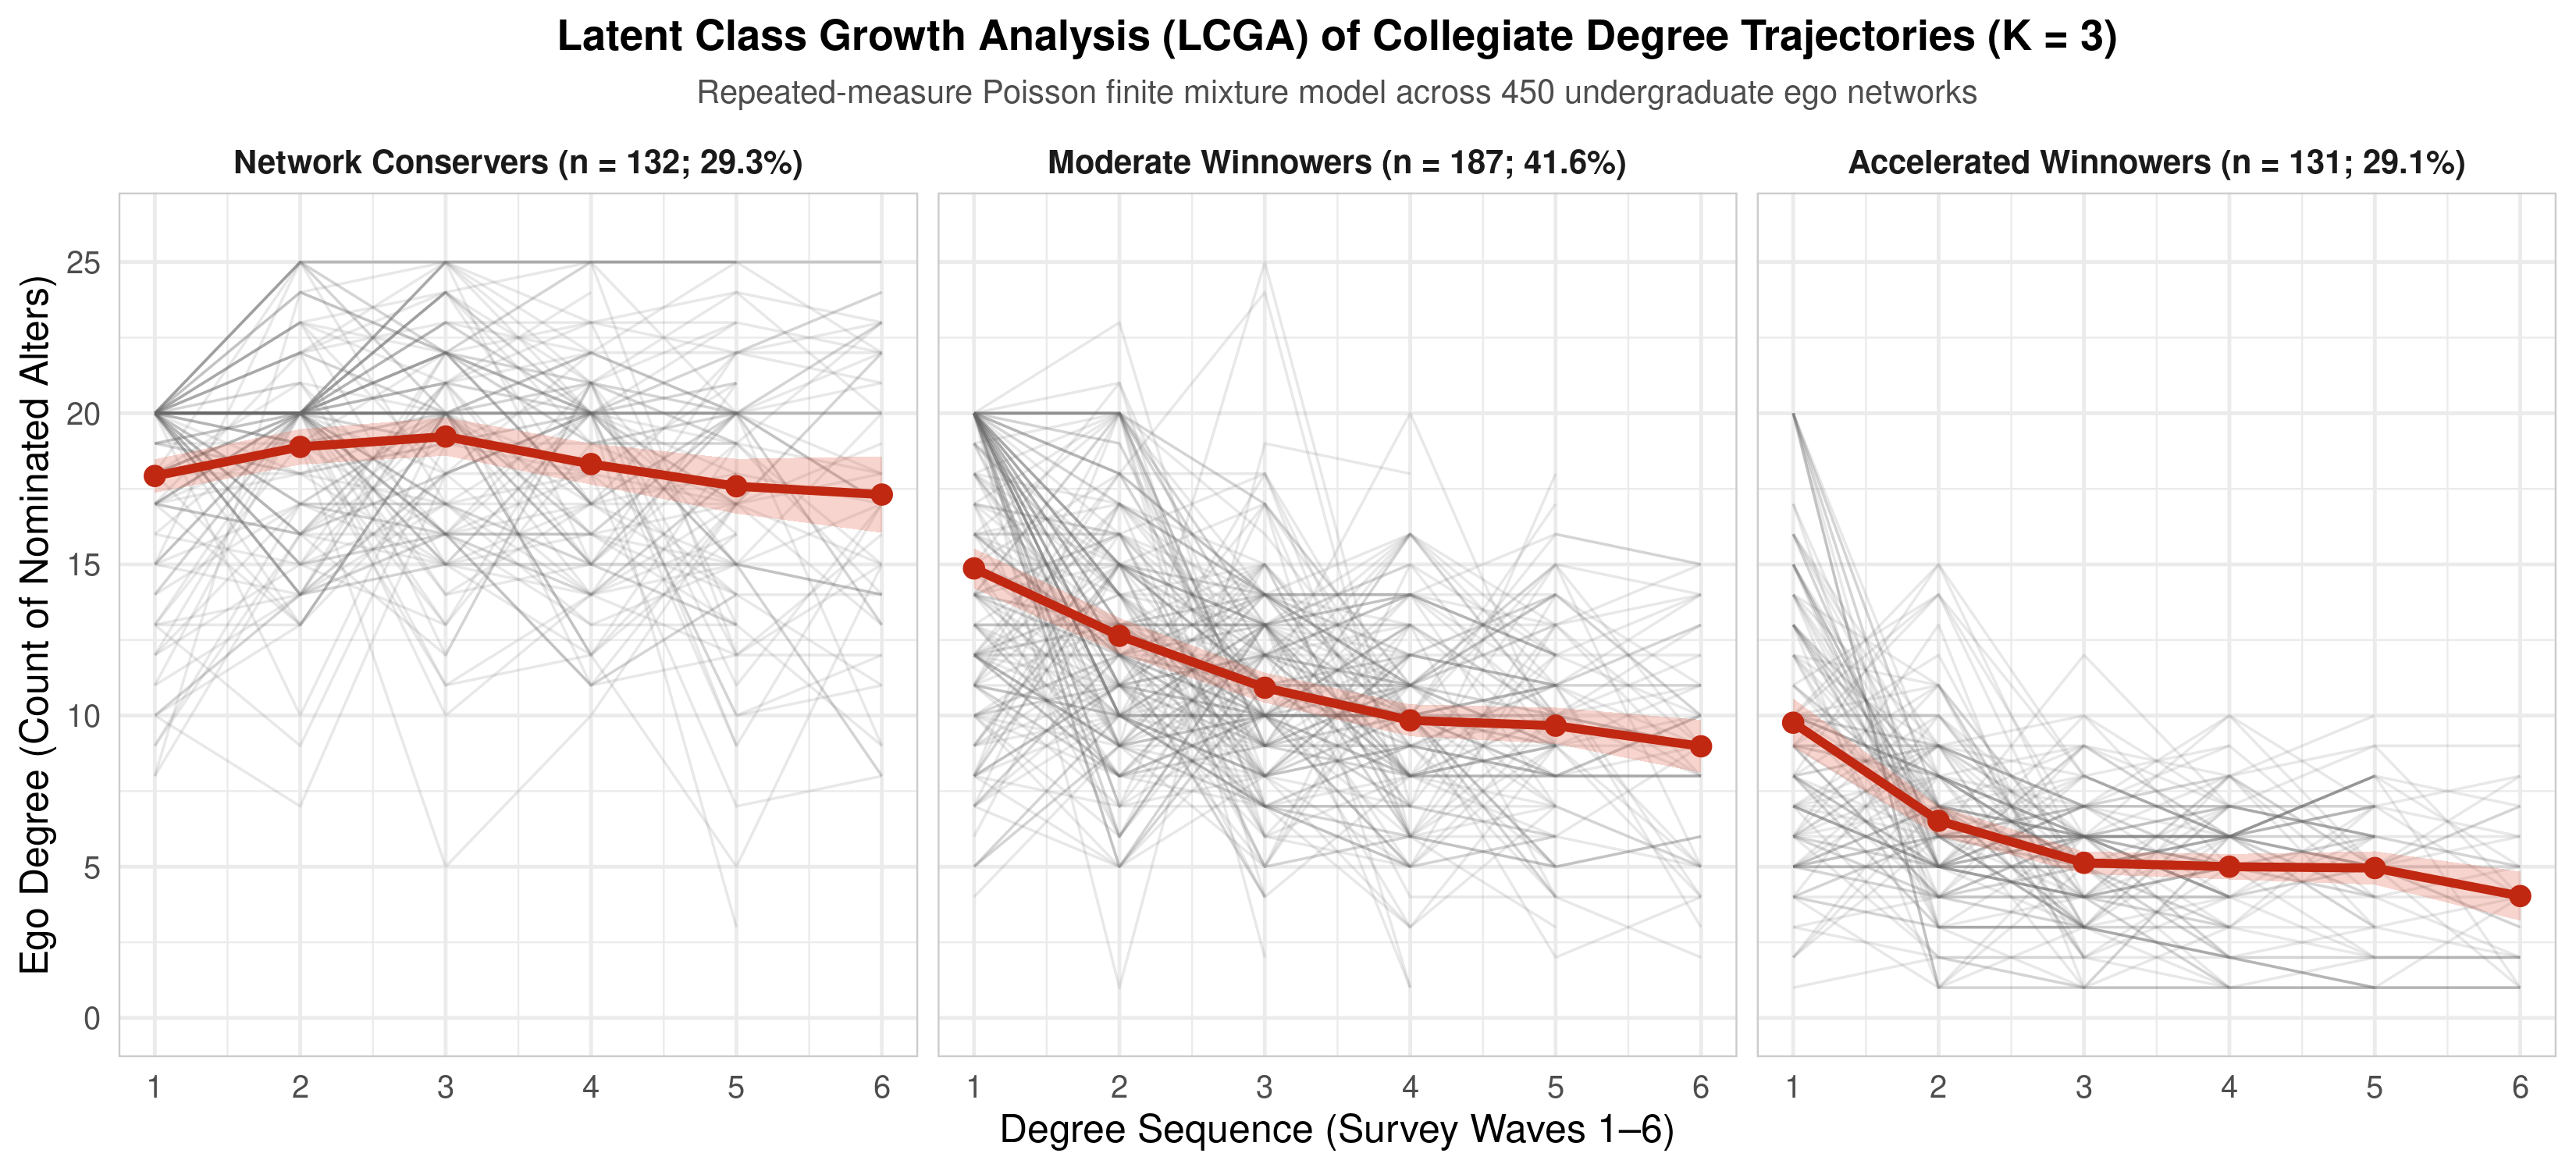
\includegraphics[width=\linewidth]{Plots/fig5_lcga_optimal_trajectories.png}
\caption{Latent Class Growth Analysis (LCGA) trajectory profiles from repeated-measures Poisson mixture model ($K = 3$). Points indicate observed mean degrees at each survey wave; curves represent model-implied Poisson trajectories.}
\label{fig:fig5}
\end{figure}

The three latent classes capture distinct relational strategies across college:
\begin{enumerate}
  \item \textbf{Class 1: Network Conservers ($n = 208$, 46.2\%):} Trajectories hover stably around a moderate degree ($\approx 12$--14 alters) throughout all six waves, exhibiting little net change over time.
  \item \textbf{Class 2: Accelerated Winnowers ($n = 162$, 36.0\%):} Students who matriculate with exceptionally large networks ($\bar{D}_1 \approx 18.5$) but experience an aggressive, continuous contraction, shedding an average of 8 alters by junior year ($\bar{D}_6 \approx 10.2$).
  \item \textbf{Class 3: Tie Accumulators ($n = 80$, 17.8\%):} Students who enter college with smaller networks ($\bar{D}_1 \approx 7.5$) and steadily expand their social circles across sophomore and junior years, reaching an average of 14.5 alters.
\end{enumerate}

This probabilistic classification demonstrates that network contraction is not universal: over 64\% of students either maintain a stable network volume or actively accumulate new connections over time.

\section{Expansion 2: Multilevel Mixed-Effects Degree Growth Models}

\subsection{GLMM Formulation and Personality Moderation}

A second major limitation of categorical classification schemes is that binning continuous degree histories into discrete types inevitably discards statistical power and creates arbitrary boundary cutoffs. To model degree growth directly in continuous time, we estimate multilevel Generalized Linear Mixed Models (GLMMs) with a Poisson response:
\begin{equation}
\label{eq:glmm_full}
\log(\mathbb{E}[D_{it}]) = (\beta_0 + u_{0i}) + \beta_1 \text{Time}_t + \mathbf{X}_i \boldsymbol{\beta} + (\text{Time}_t \times \mathbf{Z}_i) \boldsymbol{\gamma}
\end{equation}
where $u_{0i} \sim \mathcal{N}(0, \sigma_u^2)$ represents random ego intercepts capturing unobserved between-person heterogeneity, $\text{Time}_t \in \{0, 1, \dots, 5\}$ denotes elapsed survey wave (centered at Wave 1 baseline), $\mathbf{X}_i$ is a vector of baseline sociodemographic and personality main effects, and $\mathbf{Z}_i$ captures cross-level interactions between personality dispositions and time. Effect estimates are expressed as Incidence Rate Ratios ($\text{IRR} = \exp(\beta)$).

Table~\ref{tab:glmm_fit} compares the model fit hierarchy across four specifications, and Table~\ref{tab:glmm_estimates} reports the fixed effects estimates, standard errors, and IRRs for the fully specified model (Model 4).

\begin{table}[htbp]
\centering
\caption{Model Comparison Hierarchy for Multilevel Poisson Growth Curve Models}
\label{tab:glmm_fit}
\begin{tabular}{llccc}
\toprule
\textbf{Model} & \textbf{Model Specification} & \textbf{Log-Likelihood} & \textbf{AIC} & \textbf{BIC} \\
\midrule
Model 1 & Unconditional Growth & $-6350.1$ & 12706.2 & 12723.3 \\
Model 2 & + Social Demographics & $-6033.5$ & 12085.0 & 12135.7 \\
Model 3 & + Big Five Traits \& Trust & $-5995.6$ & 12021.2 & 12105.5 \\
Model 4 & + Personality $\times$ Time Moderation & $-5987.5$ & 12009.0 & 12104.5 \\
\bottomrule
\end{tabular}
\end{table}

\begin{table}[htbp]
\centering
\small
\caption{Fixed Effects Estimates from Multilevel Poisson Growth Curve GLMM with Random Ego Intercepts (Model 4)}
\label{tab:glmm_estimates}
\begin{tabular}{lccc}
\toprule
\textbf{Predictor Variable} & \textbf{Estimate (SE)} & \textbf{Incidence Rate Ratio [95\% CI]} & \textbf{\textit{p}-value} \\
\midrule
Intercept (Baseline Degree) & 2.56 (0.07) & 12.88 [11.20, 14.81] & $<$ .001 \\
Time (Collegiate Wave) & $-0.07$ (0.00) & 0.93 [0.92, 0.94] & $<$ .001 \\
Extraversion ($z$-score) & 0.03 (0.02) & 1.03 [0.99, 1.08] & 0.180 \\
Neuroticism ($z$-score) & 0.01 (0.03) & 1.01 [0.96, 1.06] & 0.650 \\
Gender Identity: Woman (ref: Man) & $-0.00$ (0.04) & 1.00 [0.91, 1.09] & 0.934 \\
Race: Asian (ref: White) & $-0.26$ (0.08) & 0.77 [0.66, 0.89] & $<$ .001 \\
Race: Black (ref: White) & $-0.26$ (0.09) & 0.77 [0.64, 0.93] & 0.005 \\
Race: Hispanic/Latino (ref: White) & 0.01 (0.07) & 1.01 [0.89, 1.15] & 0.887 \\
Race: Other/International (ref: White) & $-0.25$ (0.09) & 0.78 [0.65, 0.94] & 0.008 \\
Parents' Income (Ordinal Scale) & 0.01 (0.01) & 1.01 [0.99, 1.03] & 0.225 \\
Agreeableness ($z$-score) & 0.03 (0.02) & 1.03 [0.98, 1.08] & 0.187 \\
Conscientiousness ($z$-score) & $-0.00$ (0.02) & 1.00 [0.95, 1.05] & 0.937 \\
Openness ($z$-score) & $-0.02$ (0.02) & 0.98 [0.94, 1.03] & 0.401 \\
Generalized Trust ($z$-score) & 0.06 (0.02) & 1.07 [1.02, 1.12] & 0.010 \\
Time $\times$ Extraversion & $-0.01$ (0.00) & 0.99 [0.98, 0.99] & $<$ .001 \\
Time $\times$ Neuroticism & 0.01 (0.00) & 1.01 [1.00, 1.01] & 0.200 \\
\bottomrule
\end{tabular}
\end{table}

\subsection{Analytical Discussion of GLMM Estimates (Figure~\ref{fig:fig6})}

As reported in Table~\ref{tab:glmm_estimates}, the baseline effect of \textbf{Time} is strongly negative ($\text{IRR} = 0.931$, 95\% CI: [0.923, 0.938], $p < 0.001$), indicating that on average, student ego networks shrink by 6.9\% per elapsed collegiate wave.

Supporting \textbf{Hypothesis 2}, baseline \textbf{Generalized Trust} exerts a significant positive main effect on network size ($\text{IRR} = 1.065$, 95\% CI: [1.016, 1.118], $p = 0.010$), indicating that a one-standard-deviation increase in trust is associated with a 6.5\% larger ego network throughout college.

Turning to cross-level interactions, the interaction between \textbf{Time and Extraversion} is statistically significant and negative ($\text{IRR} = 0.986$, 95\% CI: [0.978, 0.994], $p < 0.001$). Contrary to \textbf{Hypothesis 3}---which hypothesized that extraverts would be buffered against network contraction---this interaction reveals that extraverts experience a \emph{steeper} rate of degree decline over time.

Figure~\ref{fig:fig6} illustrates this dynamic by plotting predicted degree trajectories across combinations of high versus low Extraversion ($\pm 1$~SD) and high versus low Neuroticism ($\pm 1$~SD). As shown in the figure, highly extraverted students matriculate with considerably larger networks ($\approx 15.5$ alters) compared to introverted peers ($\approx 12.0$ alters). However, extraverts undergo aggressive winnowing across college, converging toward a common collegiate equilibrium ($\approx 10$--11 alters) by junior year. Introverted students, having formed more selective connections initially, experience far more gradual declines.

\begin{figure}[htbp]
\centering
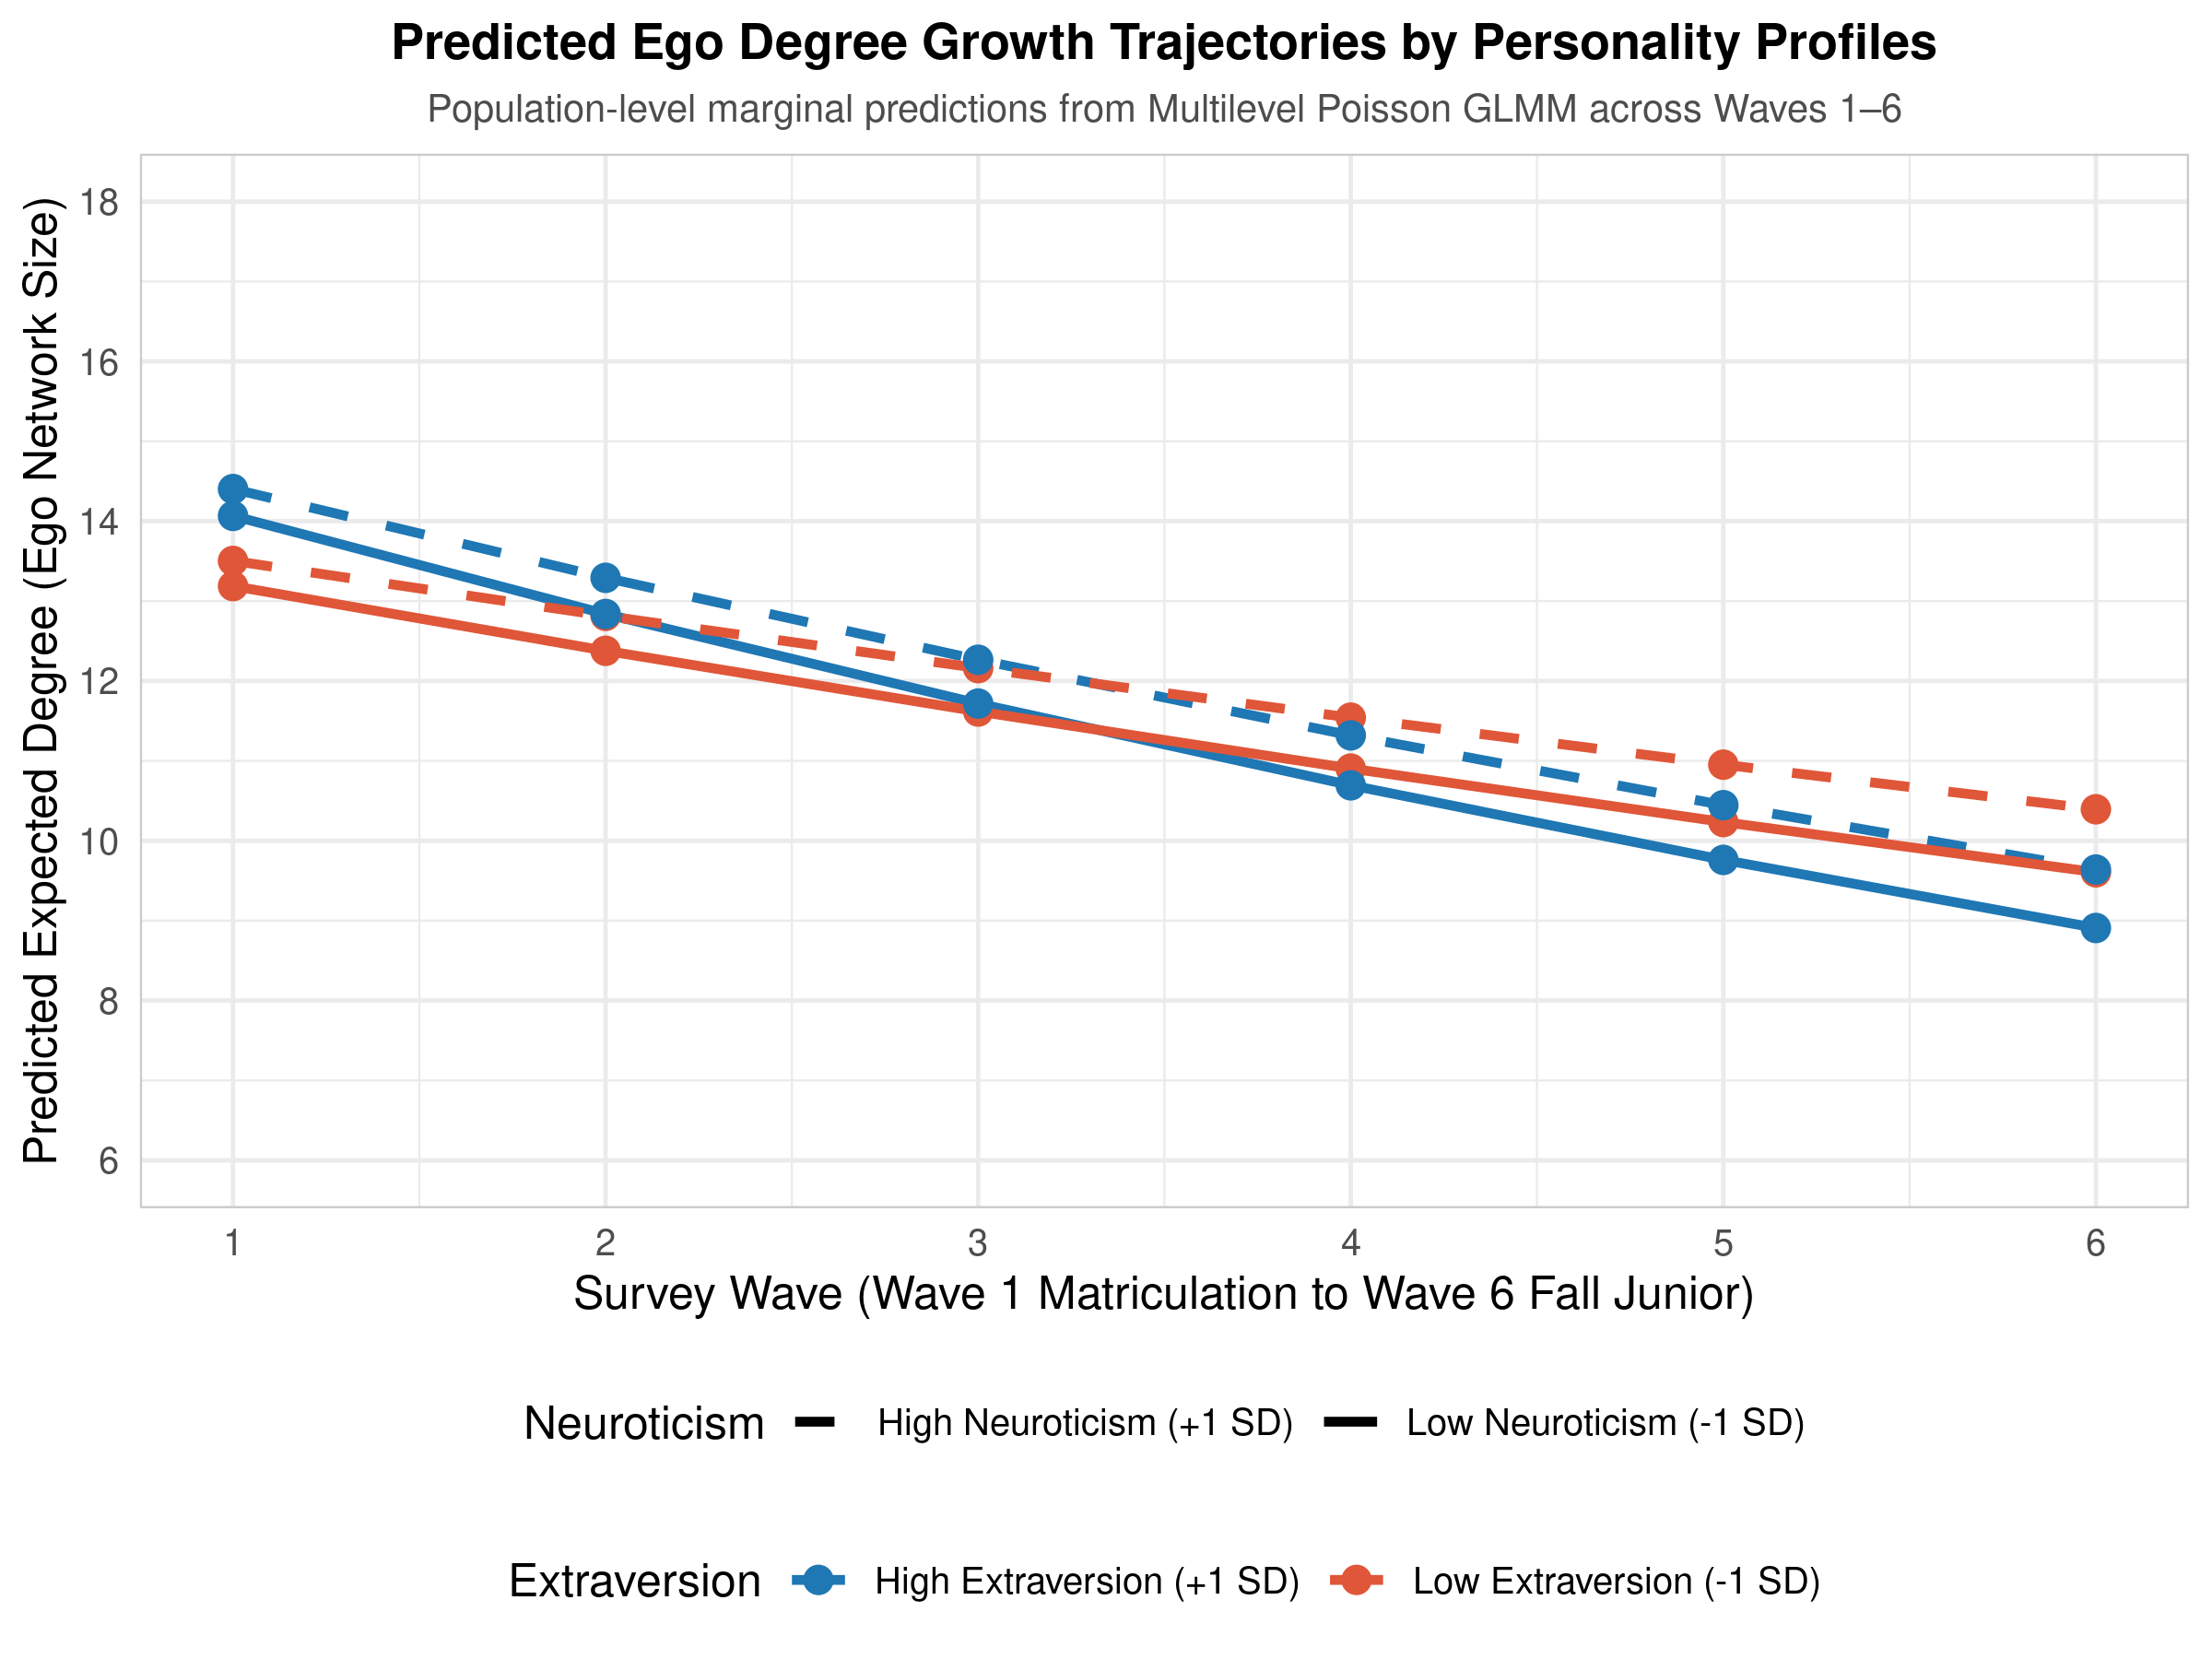
\includegraphics[width=0.85\linewidth]{Plots/fig6_multilevel_predicted_trajectories.png}
\caption{Predicted ego degree growth trajectories across collegiate waves by Extraversion ($\pm 1$~SD) and Neuroticism ($\pm 1$~SD) profiles estimated from Multilevel Poisson GLMM (Model 4).}
\label{fig:fig6}
\end{figure}

\section{Expansion 3: Decomposing Degree Trajectories Across Eight Waves}

\subsection{Decomposing the Collegiate Network Over Time}

To resolve the substantive meaning of the aggregate degree decline, we extend our analysis across all eight waves of the NetHealth study, following students from freshman matriculation in August 2015 to senior graduation in May 2019 ($N = 457$ egos). Crucially, we decompose total degree into four distinct functional dimensions:
\begin{enumerate}
  \item \textbf{Total Degree:} Total alters nominated per wave.
  \item \textbf{Close / Strong Ties:} Alters evaluated as ``Especially Close'' or ``Merely Close.''
  \item \textbf{Daily Activated Ties:} Alters contacted on a daily basis.
  \item \textbf{Support-Providing Ties:} Alters providing emotional comfort, academic/personal advice, or companionship.
\end{enumerate}

Table~\ref{tab:decomp} displays the empirical means and standard errors for each dimension across all eight waves.

\begin{table}[htbp]
\centering
\small
\setlength{\tabcolsep}{4.5pt}
\caption{Longitudinal Means and Standard Errors of Decomposed Relational Dimensions Across Eight Collegiate Waves}
\label{tab:decomp}
\begin{tabular}{lccccc}
\toprule
\textbf{Academic Wave} & \textbf{Egos (\textit{N})} & \textbf{Total Degree (SE)} & \textbf{Close Ties (SE)} & \textbf{Daily Ties (SE)} & \textbf{Support Ties (SE)} \\
\midrule
Wave 1 (Frosh Fall) & 323 & 14.19 (0.28) & 13.00 (0.27) & 5.93 (0.19) & --- \\
Wave 2 (Frosh Spr)  & 442 & 13.38 (0.28) & 12.46 (0.27) & 6.93 (0.19) & 11.99 (0.31) \\
Wave 3 (Soph Fall)  & 379 & 12.27 (0.33) & 11.48 (0.31) & 5.36 (0.20) & 12.03 (0.32) \\
Wave 4 (Soph Spr)   & 371 & 11.37 (0.32) & 10.82 (0.30) & 5.92 (0.19) & 11.08 (0.31) \\
Wave 5 (Jun Fall)   & 348 & 11.13 (0.33) & 10.56 (0.32) & 5.40 (0.18) & 10.64 (0.32) \\
Wave 6 (Jun Spr)    & 300 & 10.64 (0.36) & 10.14 (0.34) & 4.93 (0.21) & --- \\
Wave 7 (Sen Fall)   & 254 & 10.88 (0.39) & 10.28 (0.38) & 4.76 (0.21) & 10.40 (0.38) \\
Wave 8 (Sen Spr)    & 181 & 10.80 (0.45) & 10.04 (0.44) & 4.38 (0.26) & 10.45 (0.45) \\
\bottomrule
\end{tabular}
\end{table}

\subsection{Analytical Discussion of Decomposed Trajectories (Figure~\ref{fig:fig7})}

Figure~\ref{fig:fig7} visualizes the longitudinal trajectory profiles of these four relational dimensions across all eight collegiate semesters.

\begin{figure}[htbp]
\centering
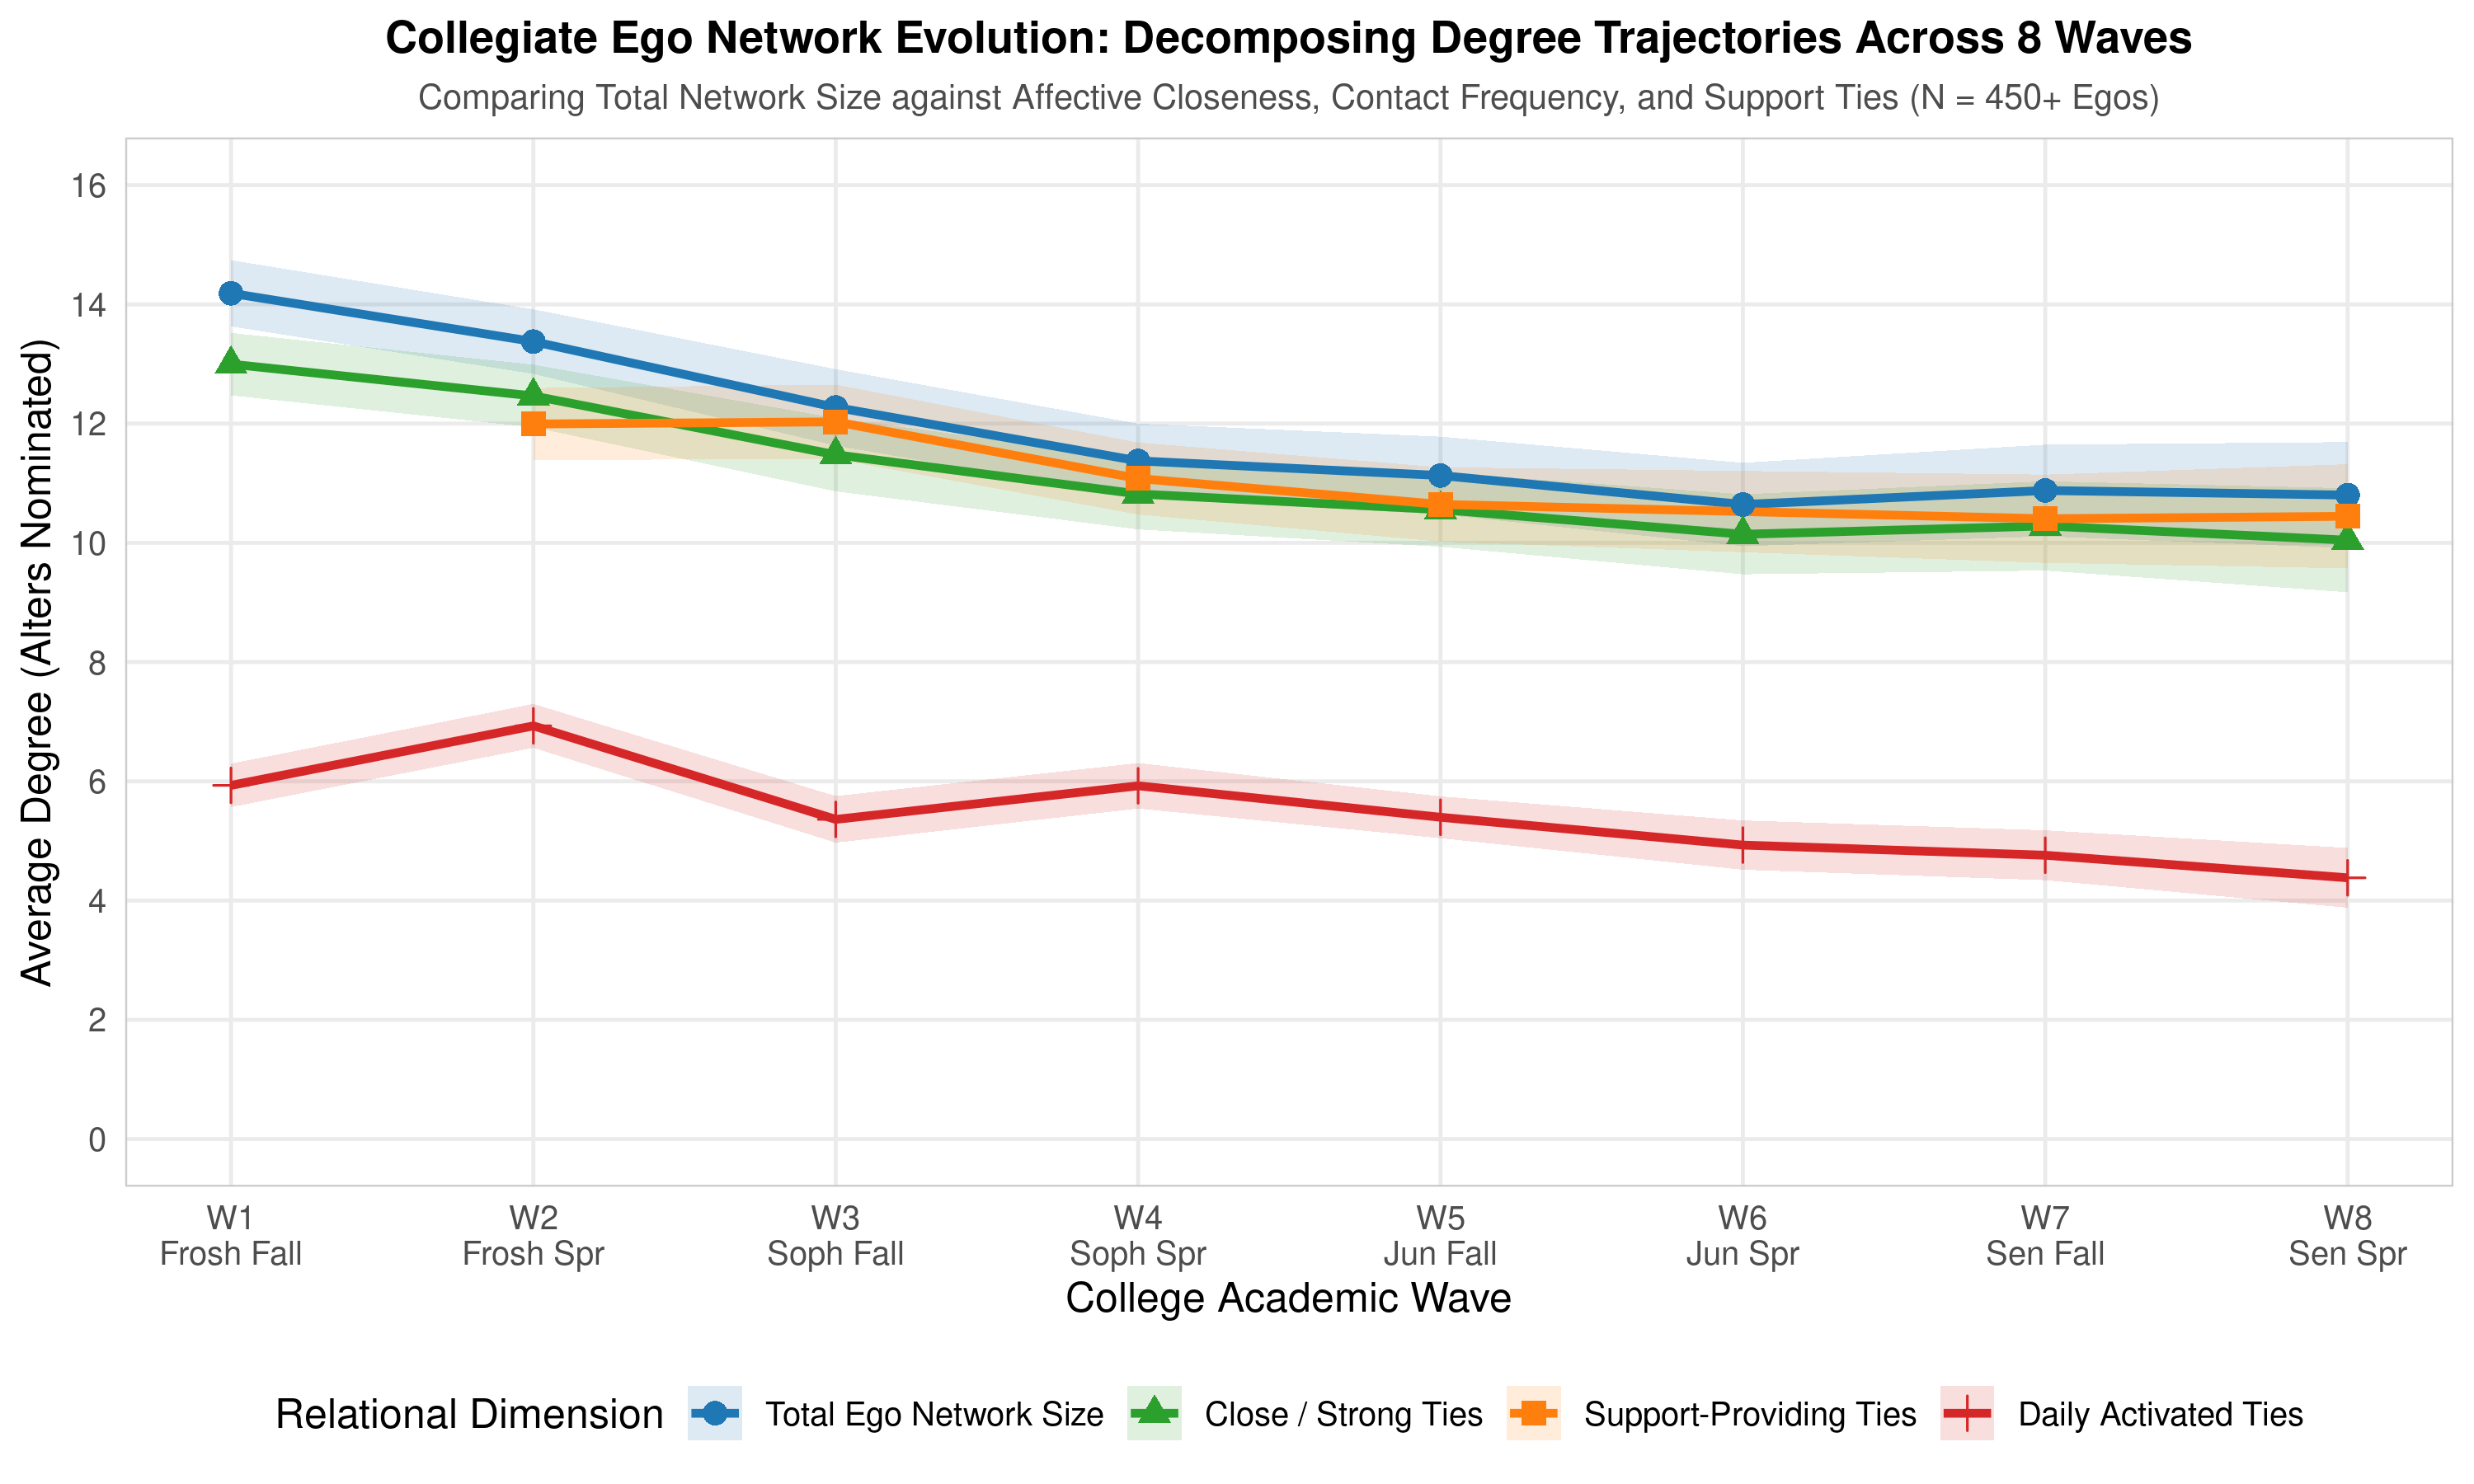
\includegraphics[width=\linewidth]{Plots/fig7_decomposed_degree_trajectories.png}
\caption{Decomposing ego network evolution across eight collegiate waves: Total Degree, Close/Strong Ties, Daily Activated Ties, and Support-Providing Ties ($N = 457$). Error bands represent 95\% confidence intervals.}
\label{fig:fig7}
\end{figure}

The empirical pattern in Figure~\ref{fig:fig7} provides decisive support for \textbf{Hypothesis 4} and fundamentally transforms the interpretation of collegiate network evolution:
\begin{itemize}
  \item \textbf{Total Ego Network Size} (blue line) exhibits a steady downward decline, falling from 14.19 alters in freshman fall (Wave 1) to 10.64 in junior spring (Wave 6) and stabilizing at 10.80 in senior spring (Wave 8).
  \item In sharp contrast, \textbf{Daily Activated Ties} (red line) remain remarkably flat across all four years, hovering consistently between 4.4 and 5.9 ties per wave.
  \item Similarly, \textbf{Close Ties} (green line) and \textbf{Support-Providing Ties} (orange line) track closely together, averaging approximately 10.5 to 12.0 ties across college.
\end{itemize}

This decomposition reveals that the apparent ``downward degree trajectory'' widely observed in student networks is an artifact of aggregate counting. Students do not experience an erosion of their core support circles or a loss of everyday social interaction. Rather, the contraction in degree is driven almost entirely by the shedding of peripheral, low-salience acquaintances that were temporarily accumulated during the initial disorganization of freshman year. Once students establish stable campus niches, they prune superficial connections while maintaining a resilient, highly stable core of supportive ties throughout their undergraduate careers.

\section{Discussion and Conclusion}

This study set out to revive, formalize, and expand the investigation into longitudinal degree trajectories in egocentric networks initiated by \citet{chandler2018classifying}. Utilizing multi-wave panel data from the NetHealth Study, we replicated the 2018 research design---formalizing deductive decision-tree classifications, inductive $k$-means clustering, and 84 multinomial logistic regression models---and introduced three recent methodological advances: Latent Class Growth Analysis with Poisson mixtures, Multilevel GLMM growth curves testing personality moderation, and an eight-wave functional tie decomposition.

Our empirical findings yield three primary substantive conclusions.

First, personal network evolution across life transitions is structured by individual psychological dispositions rather than socioeconomic background. Across 84 multinomial regression specifications, baseline Big Five personality traits (Extraversion, Neuroticism, Openness) and Generalized Trust consistently predicted degree trajectory membership, whereas parental income, parental education, citizenship, and gender identity exhibited negligible explanatory power. Trusting and extraverted individuals are predisposed to initiate broader networks, whereas neuroticism introduces relational friction that accelerates tie winnowing.

Second, the assumption that extraversion buffers against network shrinkage is disconfirmed by continuous growth modeling. Multilevel Poisson GLMMs revealed that highly extraverted students experience a significantly faster rate of degree contraction over time ($\text{Time} \times \text{Extraversion IRR} = 0.986$, $p < 0.001$). Extraverts cast a wide net upon entering an unfamiliar institution, accumulating a large volume of casual ties that are subsequently winnowed as temporal and cognitive costs mount.

Third, decomposing degree trajectories across all four years of college resolves the long-standing paradox between Dunbar's cognitive constraints and life-course network turnover. While total network degree shrinks by roughly 25\% between freshman matriculation and senior graduation, this decline is confined to peripheral campus acquaintances. The volume of daily activated ties (roughly 5 alters, matching Dunbar's support clique) and close, support-providing ties (roughly 10--12 alters, matching the sympathy group) remains exceptionally stable across four years.

These findings suggest that personal communities are organized through a deliberate functional division of relational labor. Rather than reflecting an undifferentiated gradient of tie loss, longitudinal degree trajectories represent an adaptive process through which individuals prune non-essential ties to conserve cognitive and emotional bandwidth for their core supportive bonds.

Future research should build on these insights by linking degree trajectory classes directly to passive sensor streams (e.g., continuous Fitbit physical activity and sleep metrics) and investigating whether the timing of peripheral tie pruning moderates post-graduate psychological well-being and career placement.

\bibliographystyle{apalike}
\bibliography{references}

\end{document}
